\chapter{Model-based Control of Handed Shearing Auxetics (HSA) Robots}
\label{chp:hsacontrol}

\begin{foreword}
    In Chapter~\ref{chp:hsacontrol}, we developed kinematic and dynamical models for planar \gls{HSA} robots. However, the control of \gls{HSA} remains an unexplored area, both in our previous chapters and in the existing literature. 
    We present in this chapter various model-based control approaches for planar \gls{HSA} robots ranging from PID (with integral saturation) + feedforward configuration-space control (Section~\ref{sec:hsacontrol:configuration_space_regulation}) to Cartesian-space impedance control (Section~\ref{sec:hsacontrol:task_space_impedance_control}). Notably, we rigorously validate and benchmark the proposed control strategies experimentally on two different \gls{HSA} robot prototypes.
\end{foreword}

\blfootnote{This chapter is partly based on 
    \begin{itemize}
        \item[\faFileTextO] ~\emph{\textbf{M. Stölzle}, D. Rus, and C. Della Santina (2023, December). An Experimental Study of Model-based Control for Planar Handed Shearing Auxetics Robots. In Experimental Robotics: The 18th International Symposium. Springer}~\cite{stolzle2024experimental}.
        \item[\faTrophy \, \faFileTextO] ~\emph{\textbf{M. Stölzle}*, S. S. Baberwal*, D. Rus, S. Coyle, and C. Della Santina (2024). Guiding Soft Robots with Motor-Imagery Brain Signals and Impedance Control. In Proceedings of The 2024 IEEE 7th International Conference on Soft Robotics (RoboSoft) (pp. 1-8). IEEE. Received the \textbf{Best Paper Award}~\cite{stolzle2024guiding}}.
    \end{itemize}
}

\begin{abstract}
    % Parallel robots based on Handed Shearing Auxetics (HSAs) can implement complex motions using standard electric motors while maintaining the complete softness of the structure, thanks to specifically designed architected metamaterials.
    The control of robots based on Handed Shearing Auxetics (HSAs) is especially challenging due to varying and coupled stiffness, shearing, non-affine terms in the actuation model, and underactuation. In this chapter, we present two model-based control strategies for planar HSA robots enabling regulation in task space. 
    Firstly, we propose a control strategy composed of steady-state planning for identifying a statically admittable robot shape with matching actuation and a P-satI-D feedback controller compensating elastic and gravitational forces in configuration space. 
    Secondly, we derive a task-space impedance controller that allows us to unite the soft robot's embodied intelligence with computational intelligence to guarantee compliance and interaction safety.
    We experimentally verify both proposed control strategies in closed loop.
\end{abstract}

%% Start the actual chapter on a new page.
\newpage

\section{Introduction}
% The deformability, adaptiveness, and compliance of invertebrates serve as an inspiration for continuum soft robots.
% While serial continuum soft robots have been intensively investigated in recent years~\cite{della2023model}, parallel soft robots~\cite{hughes2020extensible, zhang2020modeling} are less studied despite exhibiting exciting properties such as an improved stiffness-to-weight ratio. 
% One recent development in this field is robots based on \glspl{HSA}~\cite{truby2021recipe, kaarthik2022motorized, stolzle2024guiding} in which multiple \gls{HSA} rods are connected at their distal end through a rigid platform. 
% Twisting of the proximal end of an \gls{HSA} % with an electric actuator 
% causes the rod to elongate and enables complex motion primitives in 3D space.
Recent work has investigated proprioception~\cite{zhang2022vision}, the mechanical characterization~\cite{good2022expanding}, simulation~\cite{stolzle2023modelling}, and kinematic modeling~\cite{garg2022kinematic, stolzle2023modelling} of \gls{HSA} robots but control has yet to be tackled.
% Still, the task of control is still unsolved as \textcolor{orange}{prior work} and solutions need to be developed on how to deal with the challenges of underactuation and changing stiffness properties. 
In this work, we make a first step towards achieving task-space control by designing model-based regulators for planar motions. Our approach considers essential characteristics of \gls{HSA} robots, such as underactuation, shear strains, and varying stiffness. % and thus can serve as a building block for future research.

In Chapter~\ref{chp:hsamodel}, we derived a dynamic model for planar \gls{HSA} in Euler-Lagrange form and experimentally verified it.
We notice that the resulting planar dynamics are underactuated and that the actuation forces are non-affine with respect to the control inputs, which are the motor angles. The latter is a peculiarity of these systems, rarely observed in other robots.
Based on the model knowledge, we propose in this chapter two control strategies for planar \gls{HSA} robots capable of regulating the end-effector towards a desired position in task-space.
The first strategy, as shown in Fig.~\ref{fig:hsacontrol:configuration_space_regulation:block_scheme_closed_loop_control}, performs steady-state planning to identify an admittable configuration and steady-state control input matching the desired end-effector position and then subsequently applies a P-satI-D feedback controller~\cite{pustina2022p} on the collocated form~\cite{pustina2024input} of the system dynamics.
The second strategy, as shown in Fig.~\ref{fig:hsacontrol:task_space_impedance_control:block_scheme_closed_loop_control}, directly regulates the end-effector position using a Cartesian impedance controller that fully preserves the softness of the robot.

In summary, we state our contributions as (i) a provably stable model-based control strategy for guiding the end-effector of the robot towards a desired position in Cartesian space with a configuration-space controller that combines an integral-saturated PID with a potential shaping feedforward term, (ii) a Cartesian impedance controller that allows combining the passive compliance of the \gls{HSA} robot with active compliance in the control strategy and (iii) extensive experimental verification of both control strategies. 
A video accompanies this chapter explaining the methodology and displaying video recordings of the control experiments\footnote{\url{https://youtu.be/7PgKnE_MOsY}}.


%Structure
%\begin{enumerate}
%    \item Why soft robots
%    % \item Parallel soft robots have not been widely tested out,  have interesting characteristics such as higher bending stiffness with low weight
%    \item HSAs have this special mechanism in which the motors acts throught he stiffness of the hsa on the robot shape
%    \item Control has only been performed with PID, no model-based control. Problem of underactuation needs to be solved. Way to deal with changing stiffness characteristics
%\end{enumerate}
%
%Our contributions
%\begin{itemize}
%    \item Closed-form inverse kinematics for planar continuum robots modelled using PCS
%    \item An Euler-Lagrangian model for the dynamics of HSA robots, which is then also verified experimentally 
%    \item Proposal of a control strategy involving mapping from task-space to configuration-space and PID controller respecting the underactuation
%    \item Experiments involving Model-based regulation of HSA robots
%\end{itemize}
\section{Configuration Space Regulation}\label{sec:hsacontrol:configuration_space_regulation}
In this Section, we derive a model-based control strategy in configuration space for achieving setpoint regulation that combines an integral-saturated PID controller with a potential-shaping feedforward term. We first introduce the dynamical model of the planar \gls{HSA} robot and then present the control strategy.
Subsequently, we present a steady-state planning procedure to identify admittable configurations and matching steady-state actuation.
Finally, we experimentally verify the proposed control strategy in closed loop.

\subsection{Background: Dynamical model}\label{sub:hsacontrol:model}
As introduced in Sec.~\ref{sec:hsamodel:planar_hsa_robot_model}, the state of a planar \gls{HSA} robot at time $t$ can be therefore described by $x(t) = \begin{bmatrix}
    q^\mathrm{T}(t) & \dot{q}^\mathrm{T}
\end{bmatrix}^\mathrm{T} \in \mathbb{R}^6$, where $\kappa_\mathrm{be}$, $\sigma_\mathrm{sh}$, and $\sigma_\mathrm{ax}$ denote the bending, shear, and axial strain respectively.
The dynamical model is then given in Euler-Lagrange form as
\begin{equation}\label{eq:hsacontrol:dynamics}
    M(q) \Ddot{q} + C(q,\dot{q})\dot{q} + G(q) + K (q - q^0) + D \dot{q} = \alpha(q,\phi),
\end{equation}
where $M(q),C(q,\dot{q}),K,D \in \mathbb{R}^{3 \times 3}$ are the inertia, Coriolis, elastic and damping matrices, respectively. $q^0 \in \mathbb{R}^3$ captures the rest configuration. The terms $G(q)$ and $\alpha(q,\phi) \in \mathbb{R}^3$ describe the gravitational and actuation forces acting on the generalized coordinates.
We provide examples in Fig.~\ref{fig:hsacontrol:kinematics:workspace} of the operational workspace that can be achieved with this kinematic model.
We stress that (a) the derived dynamical model is not affine in the control input and (b) the system is underactuated.

\begin{figure}[ht]
    \centering
    \subfigure[Blockscheme]{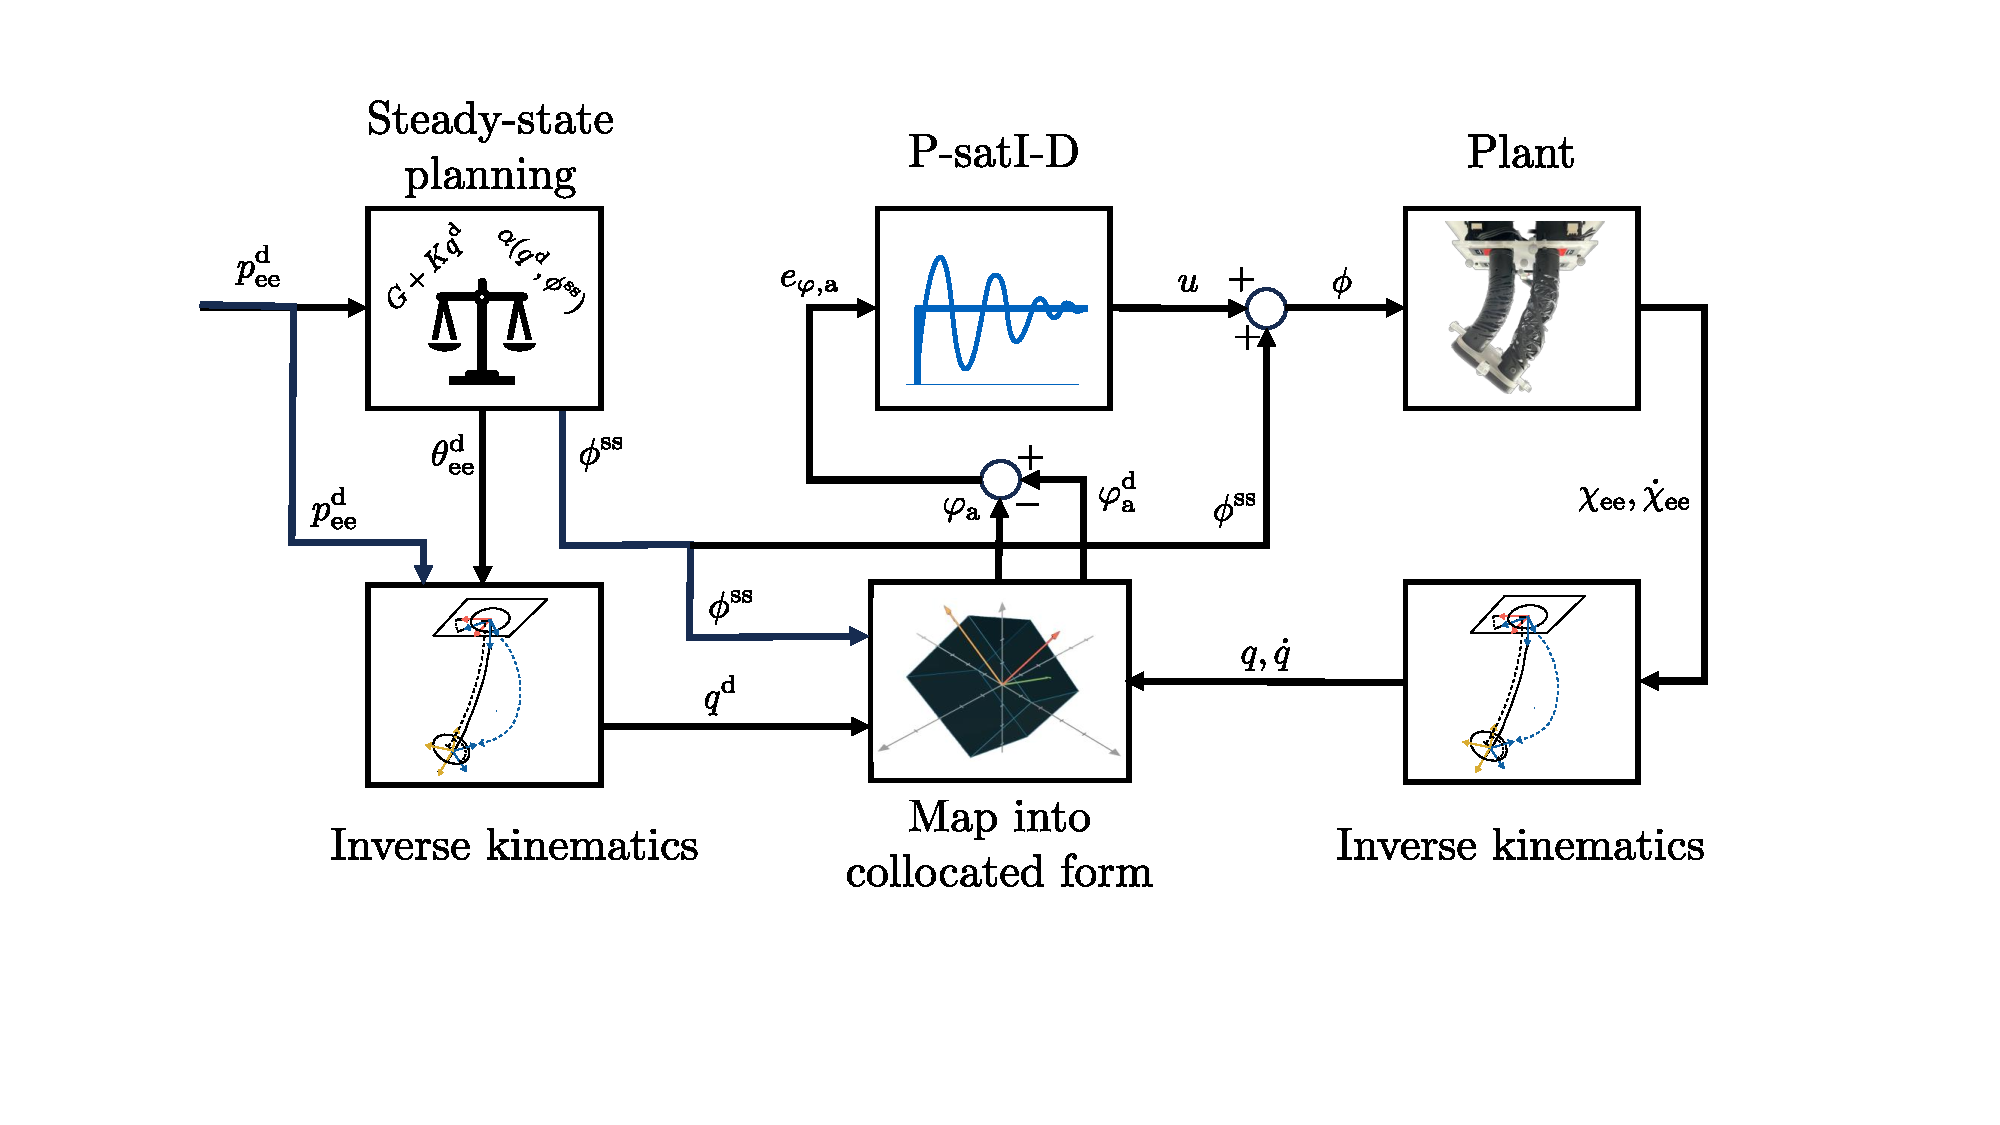
\includegraphics[width=0.62\textwidth]{hsacontrol/figures/control_schemes/configuration_space_regulation/control_scheme_v4_cropped.pdf}\label{fig:hsacontrol:configuration_space_regulation:block_scheme_closed_loop_control}}
    \subfigure[Operational workspace]{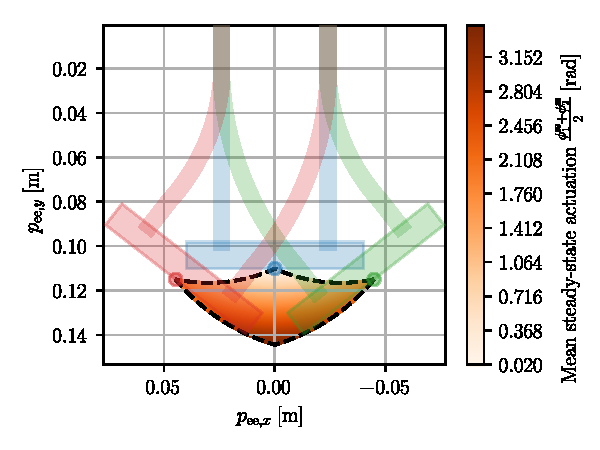
\includegraphics[width=0.37\columnwidth, trim={7, 7, 7, 7}]{hsacontrol/figures/kinematics/fpu_operational_workspace.pdf}\label{fig:hsacontrol:kinematics:workspace}}
    \caption{\textbf{Panel (a):} Block scheme for configuration-space regulator: we plan the steady-state behavior such that the end-effector matches the given desired position $p_\mathrm{ee}^\mathrm{d}$. The outputs of this planning are the steady-state actuation $\phi^\mathrm{ss}$ and a suitable end-effector orientation $\theta_\mathrm{ee}^\mathrm{d}$. After leveraging inverse kinematics to identify the desired and current configuration, $q$ is mapped into a collocated form where the inputs are decoupled. Finally, we use a P-satI-D feedback controller on the actuation coordinates $\varphi$. \textbf{Panel (b):} Visualization of the operational workspace of a planar HSA robot consisting of FPU rods. The colored area within the black dashed borders represents the positions the end-effector (visualized as a dot) can reach. The coloring denotes the mean magnitude of actuation (i.e., twisting of the rods). Furthermore, we plot three sample configurations: the unactuated straight configuration $q = [0, 0, 0]^\mathrm{T}$ (blue), maximum clockwise bending $q = [\SI{-11.2}{rad \per m}, 0.08, 0.30]^\mathrm{T}$ (red), and maximum counter-clockwise bending $q = [\SI{11.2}{rad \per m}, -0.08, 0.30]^\mathrm{T}$ (green).}
\end{figure}

\subsection{Control strategy}\label{sub:hsacontrol:configuration_space_regulation:control_strategy}

Our goal is to control the end-effector, which is defined as the distal surface of the platform, to a desired position in Cartesian space $p_\mathrm{ee}^\mathrm{d} \in \mathbb{R}^2$. 
However, the mapping into configuration space is not trivial as we do not know which end-effector orientation $\theta_\mathrm{ee}$ is feasible at steady-state. 
To tackle this challenge, we perform steady-state planning identifying admittable configurations $q^\mathrm{d}$ and matching steady-state actuations $\phi^\mathrm{ss}$, which allow the robot's end-effector to statically remain at $p_\mathrm{ee}^\mathrm{d}$. More details on the used planning procedure can be found in Section~\ref{sub:hsacontrol:experiments:steady_state_planning}.

\begin{figure}[hbt]
    \centering
    \subfigure[$\alpha(q, \phi)$ for FPU]{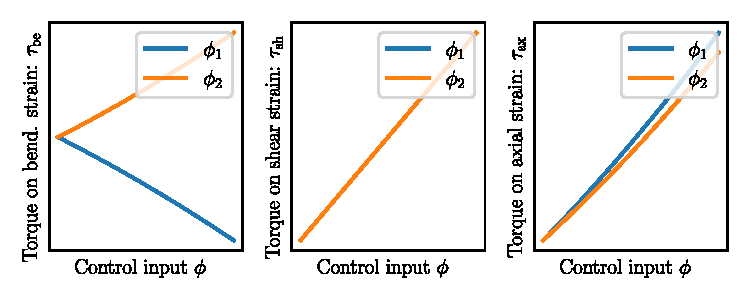
\includegraphics[width=0.80\columnwidth]{hsacontrol/figures/actuation_characteristics/nonlinear_alpha_fpu_cropped.pdf}}\\
    \subfigure[$\alpha(q, \phi)$ for EPU]{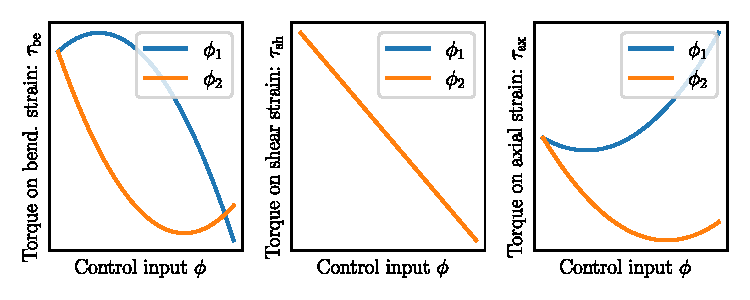
\includegraphics[width=0.80\columnwidth]{hsacontrol/figures/actuation_characteristics/nonlinear_alpha_epu_cropped.pdf}}\\
    \subfigure[$\alpha(q^\mathrm{ss}, \phi^\mathrm{ss}) + A_{\phi^\mathrm{ss}}(q) \, (\phi - \phi^\mathrm{ss})$ for EPU]{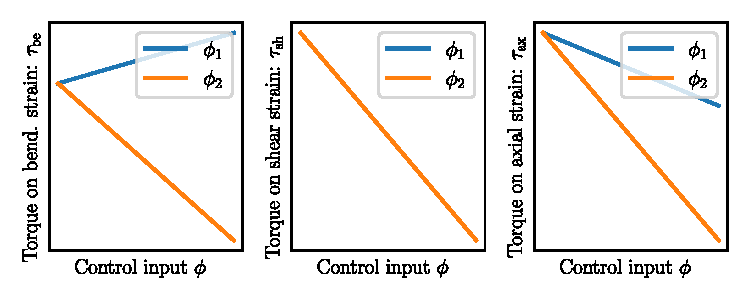
\includegraphics[width=0.80\columnwidth]{hsacontrol/figures/actuation_characteristics/linearized_alpha_epu_cropped.pdf}}\\
    \subfigure[$A_{\varphi} \, (\phi - \phi^\mathrm{ss})$]{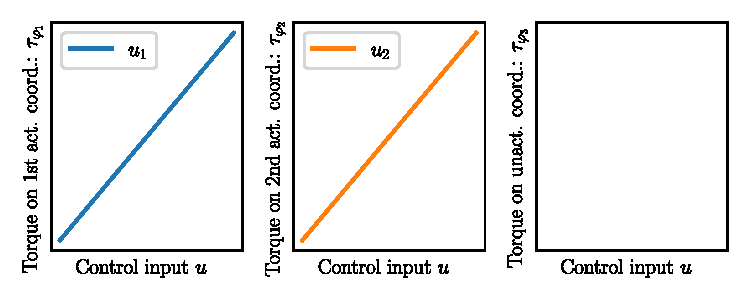
\includegraphics[width=0.80\columnwidth]{hsacontrol/figures/actuation_characteristics/actuation_coordinates_cropped.pdf}}\\
    \caption{Mapping of actuation $\phi \in \mathbb{R}^2$ to configuration-space torques $\tau \in \mathbb{R}^3$ for planar \gls{HSA} robots. The first two rows visualize the modeled nonlinear, coupled mapping for the FPU and EPU materials, respectively. The third row illustrates the mapping for a linearized actuation term. Finally, in actuation coordinates, the mapping is fully decoupled, as shown in the fourth row.}
    \label{fig:hsacontrol:actuation_characteristics}
\end{figure}

In principle, we can command $\phi = \phi^\mathrm{ss}$ to achieve regulation towards the desired end-effector position.
Nevertheless, we add a feedback controller to compensate for any errors in $\phi^\mathrm{ss}$ caused by unmodelled effects such as hysteresis. Unfortunately, as illustrated in Fig.~\ref{fig:hsacontrol:actuation_characteristics}, the non-affine actuation $\alpha(q,\phi)$ would complicate the design of such a feedback controller.
% Now, we can regulate the robot in configuration space towards $q^\mathrm{d}$. However, we notice that our system is non-affine in the control input $\phi$. 
Therefore, we perform a first-order Taylor expansion of the actuation forces with respect to $\phi$ resulting in a configuration-dependent actuation matrix $A_{\phi^\mathrm{ss}}(q) = \frac{\partial \alpha}{\partial \phi} \big|_{\phi = \phi_\mathrm{ss}} \in \mathbb{R}^{3 \times 2}$. This allows us to re-write the right side of the \gls{EOM} as $\tau_q = \alpha(q^\mathrm{ss}, \phi^\mathrm{ss}) + A_{\phi^\mathrm{ss}}(q) \, u$ where $u = \phi - \phi^\mathrm{ss}$ is the new control input.
% We remark that $\alpha(q^\mathrm{ss}, \phi^\mathrm{ss})$ is already compensating for the gravitational and elastic forces at the desired configuration. 
To improve the robustness of the control loop, we compute $u$ with a P-satI-D control law~\cite{pustina2022p}. However, our system is underactuated and in a non-collocated form.
Therefore, we apply a coordinate transformation $h: q \rightarrow \varphi \in \mathbb{R}^3$ recently introduced by Pustina et al.~\cite{pustina2024input} which maps the \gls{EOM} into a form where $\phi$ applies direct forces on the actuated configuration variables. The map is given by { $h(q) = \begin{bmatrix}
    \int_0^t \dot{q}^\mathrm{T} A_{\phi^\mathrm{ss}}(q) \mathrm{d}\tau, & \sigma_\mathrm{sh}
\end{bmatrix}^\mathrm{T} = \begin{bmatrix}
    h_1(q), & h_2(q), & \sigma_\mathrm{sh}
\end{bmatrix}^\mathrm{T}$}
with
\begin{footnotesize}
\begin{multline}\footnotesize
    h_i(q) = 
    C_{\mathrm{S},\mathrm{ax}} \, \frac{h_i}{l^0} \, \Big [ 2 \, \varepsilon_i(\phi^\mathrm{ss}_i) \left ( \pm r_\mathrm{off} \kappa_\mathrm{be} + \sigma_\mathrm{ax} \right ) \mp r_\mathrm{off}^2 \frac{\kappa_\mathrm{be}^2}{2} \pm r_\mathrm{off} \, \sigma_\mathrm{ax}^0 \, \kappa_\mathrm{be} \mp r_\mathrm{off} \, \kappa_\mathrm{be} \, \sigma_\mathrm{ax} + \sigma_\mathrm{ax}^0 \, \sigma_\mathrm{ax}\\ - \frac{\sigma_\mathrm{ax}^2}{2} \Big ] 
    + C_{\mathrm{S},\mathrm{b}} \, \frac{h_i}{l^0} \, \Big [ \kappa_\mathrm{be}^0 \, \kappa_\mathrm{be} - \frac{\kappa_\mathrm{be}^2}{2} \Big ] 
    + C_{\mathrm{S},\mathrm{sh}} \, \frac{h_i}{l^0} \, \Big [\sigma_\mathrm{sh}^0 \, \sigma_\mathrm{sh} - \frac{\sigma_\mathrm{sh}^2}{2} \Big ]
    + \hat{S}_\mathrm{ax} \, \frac{h_i}{l^0} \, C_\varepsilon \Big [ \pm r_\mathrm{off} \, \kappa_\mathrm{be} + \sigma_\mathrm{ax} \Big ].
\end{multline}
\end{footnotesize}
% \begin{equation}\tiny
%     \begin{bmatrix}
%          \frac{h_{1} \cdot \left(2 C_{S a1} C_\varepsilon h_{1} \phi_{1} roff_{1} \kappa_\mathrm{be} + 2 C_{S a1} C_\varepsilon h_{1} \phi_{1} \sigma_\mathrm{ax} - \frac{C_{S a1} l_{1} roff_{1}^{2} \kappa_\mathrm{be}^{2}}{2} + C_{S a1} l_{1} roff_{1} \sigma_\mathrm{ax}^0 \kappa_\mathrm{be} - C_{S a1} l_{1} roff_{1} \kappa_\mathrm{be} \sigma_\mathrm{ax} + C_{S a1} l_{1} \sigma_\mathrm{ax}^0 \sigma_\mathrm{ax} - \frac{C_{S a1} l_{1} \sigma_\mathrm{ax}^{2}}{2} + C_{S b1} \kappa_{b eq1} l_{1} \kappa_\mathrm{be} - \frac{C_{S b1} l_{1} \kappa_\mathrm{be}^{2}}{2} + C_{S sh1} l_{1} \sigma_\mathrm{sh}^0 \sigma_\mathrm{sh} - \frac{C_{S sh1} l_{1} \sigma_\mathrm{sh}^{2}}{2} + C_\varepsilon S_{a hat1} l_{1} roff_{1} \kappa_\mathrm{be} + C_\varepsilon S_{a hat1} l_{1} \sigma_\mathrm{ax}\right)}{l_{1}^{2}}\\
%          \frac{h_{2} \cdot \left(2 C_{S a2} C_\varepsilon h_{2} \phi_{2} roff_{2} \kappa_\mathrm{be} + 2 C_{S a2} C_\varepsilon h_{2} \phi_{2} \sigma_\mathrm{ax} - \frac{C_{S a2} l_{1} roff_{2}^{2} \kappa_\mathrm{be}^{2}}{2} + C_{S a2} l_{1} roff_{2} \sigma_\mathrm{ax}^0 \kappa_\mathrm{be} - C_{S a2} l_{1} roff_{2} \kappa_\mathrm{be} \sigma_\mathrm{ax} + C_{S a2} l_{1} \sigma_\mathrm{ax}^0 \sigma_\mathrm{ax} - \frac{C_{S a2} l_{1} \sigma_\mathrm{ax}^{2}}{2} + C_{S b2} \kappa_{b eq2} l_{1} \kappa_\mathrm{be} - \frac{C_{S b2} l_{1} \kappa_\mathrm{be}^{2}}{2} + C_{S sh2} l_{1} \sigma_\mathrm{sh}^0 \sigma_\mathrm{sh} - \frac{C_{S sh2} l_{1} \sigma_\mathrm{sh}^{2}}{2} + C_\varepsilon S_{a hat2} l_{1} roff_{2} \kappa_\mathrm{be} + C_\varepsilon S_{a hat2} l_{1} \sigma_\mathrm{ax}\right)}{l_{1}^{2}}\\
%          \sigma_\mathrm{sh}
%     \end{bmatrix}
% \end{equation}
The Jacobian $J_\mathrm{h}(q) = \frac{\partial h}{\partial q}$ is used to formulate the dynamics $M_\varphi \ddot{\varphi} + \eta(\varphi, \dot{\varphi}) + G_\varphi + K_\varphi + D_\varphi \, \dot{\varphi} = J_\mathrm{h}^\mathrm{-T}(q) \, \alpha(q^\mathrm{ss},\phi^\mathrm{ss}) + A_\varphi \, u $ in the collocated variables~\cite{khatib1987unified}, where $A_\varphi^\mathrm{T} = \begin{bmatrix}
    \mathbb{I}^{2} & 0^\mathrm{2 \times 1}
\end{bmatrix}^\mathrm{T}$. In the following, we will denote with the subscript $a$ the first two actuated coordinates $\varphi_\mathrm{a}$.
% 
Finally, the full control law of the \emph{P-satI-D} is given in collocated form as
\begin{equation}\label{eq:hsacontrol:gravity_compensation_controller}
    \phi = \phi^\mathrm{ss} + K_\mathrm{p} (\varphi_\mathrm{a}^\mathrm{d} - \varphi) - K_\mathrm{d} \dot{\varphi}_\mathrm{a} + K_\mathrm{i} \int_0^t \tanh(\gamma \, ( \varphi_{\mathrm{a},t'}^\mathrm{d}-\varphi_{\mathrm{a},t'})) \: \mathrm{d} t',
\end{equation}
where $K_\mathrm{p}, K_\mathrm{d}, K_\mathrm{i} \in \mathbb{R}^{2 \times 2}$ are the proportional, derivative, and integral gains respectively, and $\gamma \in \mathbb{R}^{2 \times 2}$ horizontally compresses the hyperbolic tangent. While the proposed P-satI-D control law compensates gravity through $\phi^\mathrm{ss}$, we can extend the approach to include gravity cancellation (\emph{P-satI-D + GC}) by evaluating $G_{\varphi,\mathrm{a}}$ at the current configuration:
\begin{equation}\label{eq:hsacontrol:gravity_cancellation_controller}
    \phi = \phi^\mathrm{ss} - G_{\varphi,\mathrm{a}}(q^\mathrm{d}) + G_{\varphi,\mathrm{a}}(q) + K_\mathrm{p} (\varphi_\mathrm{a}^\mathrm{d} - \varphi) - K_\mathrm{d} \dot{\varphi}_\mathrm{a} + K_\mathrm{i} \int_0^t \tanh(\gamma \, ( \varphi_{\mathrm{a},t'}^\mathrm{d}-\varphi_{\mathrm{a},t'})) \: \mathrm{d} t'.
\end{equation}
The implementation of all control laws is available on GitHub\footnote{\url{https://github.com/tud-phi/hsa-planar-control}}.

\subsection{Steady-state planning}\label{sub:hsacontrol:experiments:steady_state_planning}
Our approach, as detailed in Section~\ref{sub:hsacontrol:configuration_space_regulation:control_strategy}, requires us for a given desired end-effector position $p_\mathrm{ee}^\mathrm{d}$ to identify a statically-feasible configuration $q^\mathrm{d}$ with the matching steady-state actuation $\phi^\mathrm{ss}$.

\begin{figure}[hbt]
    \centering
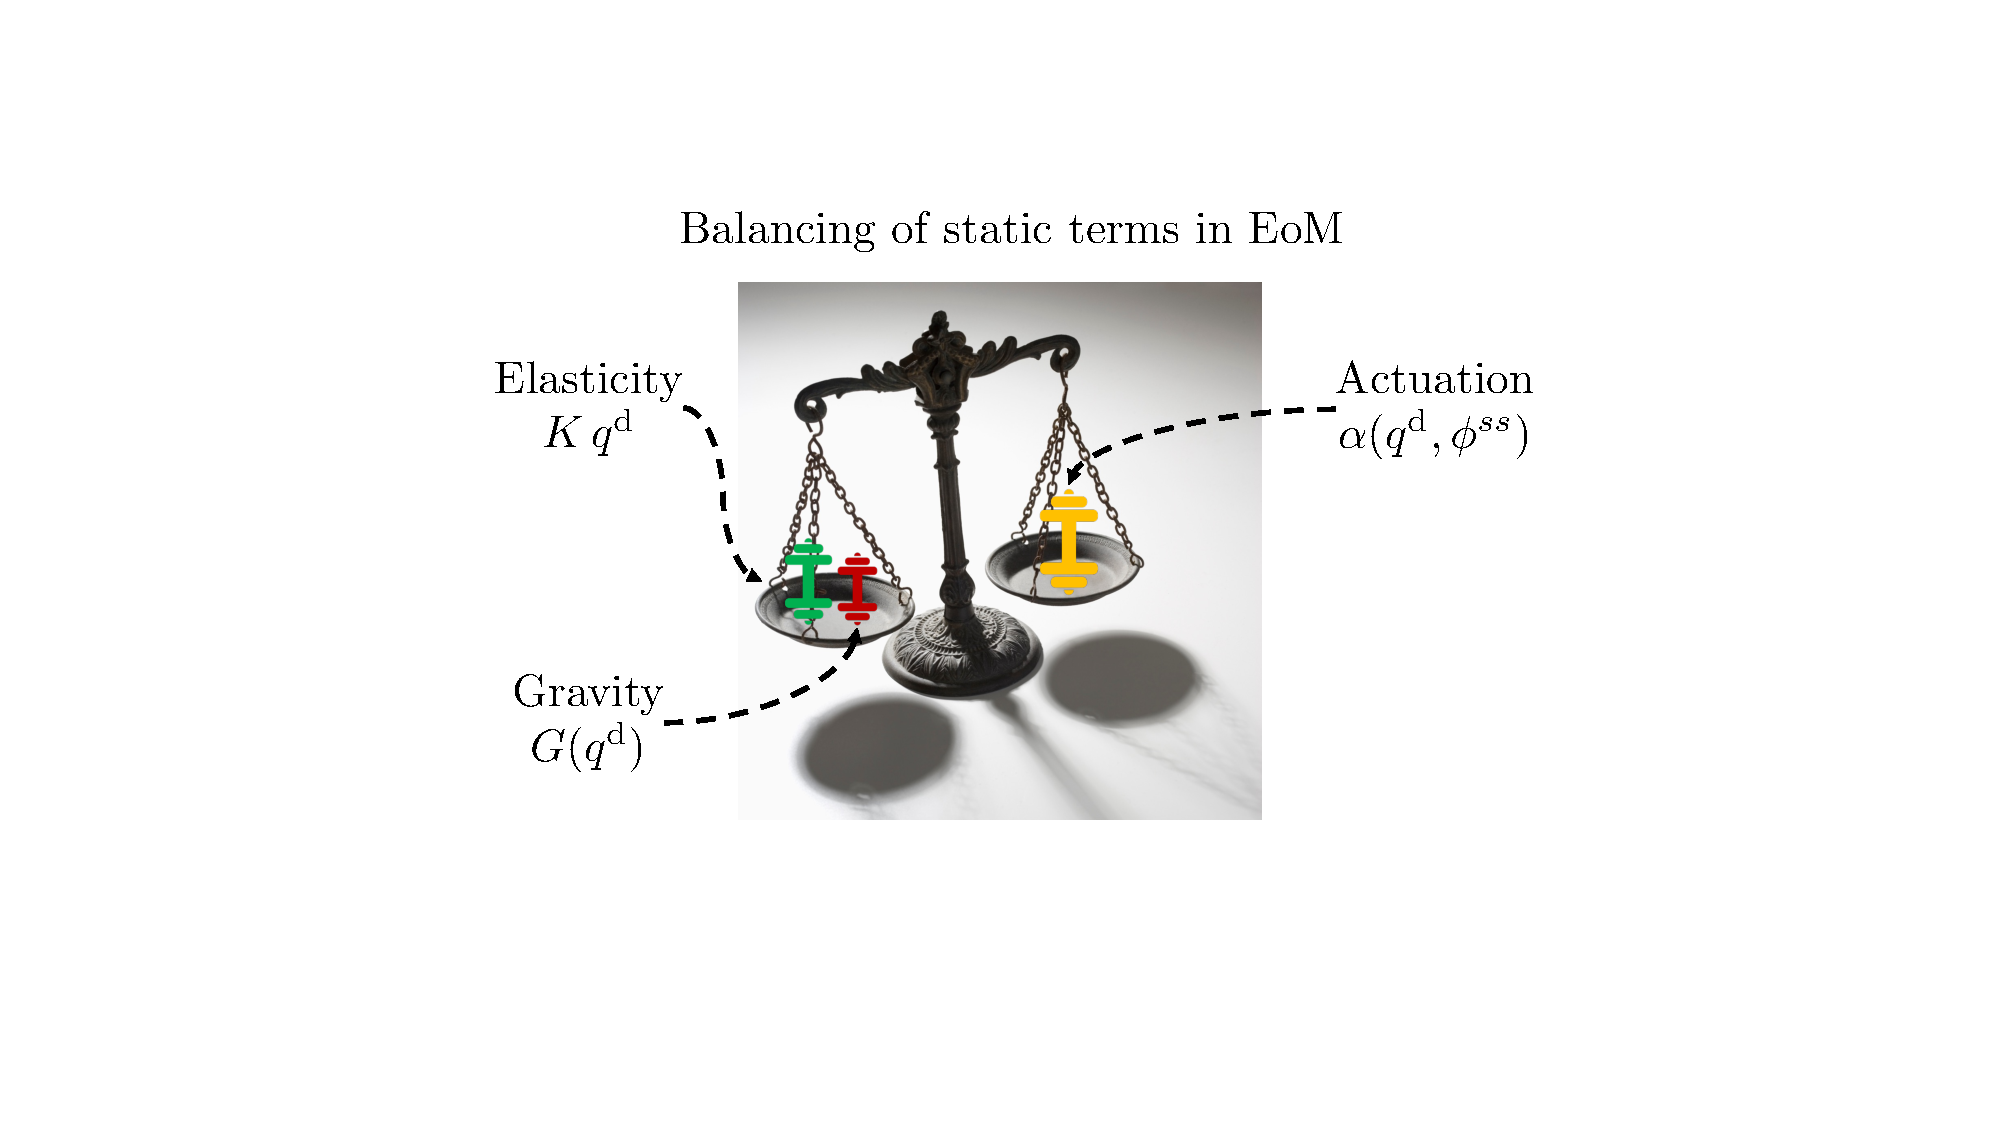
\includegraphics[width=0.5\textwidth]{hsacontrol/figures/control_schemes/configuration_space_regulation/steady_state_planning_cropped.pdf}
    \caption{Illustration of the idea behind steady-state planning: we balance the static forces that are acting at steady-state on the robot with torques generated by a steady-state actuation $\phi^\mathrm{ss}$.}
    \label{fig:hsacontrol:configuration_space_regulation:steady_state_planning}
\end{figure}

We perform online static inversion to identify admittable desired configurations $q^\mathrm{d}$ and matching steady-state control inputs $\phi^\mathrm{ss}$ during our experiments involving the FPU \gls{HSA} robots. First, we substitute the inverse kinematics $\varrho_\mathrm{ee}(\chi_\mathrm{ee})$ into the static \gls{EOM}. Then, as illustrated in Fig~\ref{fig:hsacontrol:configuration_space_regulation:steady_state_planning}, we find the roots of the equation $G\circ\varrho_\mathrm{ee}(\chi_\mathrm{ee}^\mathrm{d}) + K\circ\varrho_\mathrm{ee}(\chi_\mathrm{ee}^\mathrm{d})-\alpha(\varrho_\mathrm{ee}(\chi_\mathrm{ee}^\mathrm{d}), \phi_\mathrm{ss})$ with respect to $(\theta_\mathrm{ee},\phi_1, \phi_2)$ using nonlinear least-squares while enforcing constraints on the sign of $\phi$. We solve this optimization problem with projected gradient descent.

In contrast, the static inversion optimization problem is not well-behaved for the identified EPU system parameters. Instead, we rely on rolling out the dynamics over a duration $t_\mathrm{ss}$ to steady-state and then optimize the steady-state input $\phi^\mathrm{ss}$ such that the final end-effector error $\lVert p_\mathrm{ee}^\mathrm{d} - p_\mathrm{ee}^\mathrm{ss} \rVert$ is as small as possible. We formalize this optimization problem in a least-squares fashion
\begin{equation}\label{eq:hsacontrol:steady_state_rollout_optim_problem}
\begin{aligned}
    \phi^\mathrm{ss} = \argmin_\mathrm{\phi} \quad & \frac{1}{2} \, \lVert p_\mathrm{ee}^\mathrm{d} - p_\mathrm{ee}^\mathrm{ss}(\phi) \rVert_2^2,\\
    \textrm{s.t.} \quad & x^\mathrm{ss} = x(t_0) + \int_{t_0}^{t_\mathrm{ss}} f(x(t), \phi) \, \mathrm{d}t, \quad \chi_\mathrm{ee}^\mathrm{ss} = \begin{bmatrix}
        p_\mathrm{ee}^\mathrm{ss}\\
        \theta_\mathrm{ee}^\mathrm{ss}
    \end{bmatrix} = \pi_\mathrm{ee}(q^\mathrm{ss}),\\
\end{aligned}
\end{equation}
where $\dot{x}(t) = f(x(t), \phi)$ are the nonlinear state-space dynamics based on the \gls{EOM} derived in Section~\ref{sub:hsamodel:planar_hsa_robot_model:dynamics} and $\phi \in \mathbb{R}^2$ is constant in time. We solve \eqref{eq:hsacontrol:steady_state_rollout_optim_problem} online using the Levenberg-Marquardt algorithm. Finally, we choose $q^d = q^\mathrm{ss}$ and $\chi_\mathrm{ee}^\mathrm{d} = \pi_\mathrm{ee}(q^d)$.

\begin{figure}[t]
    \centering
    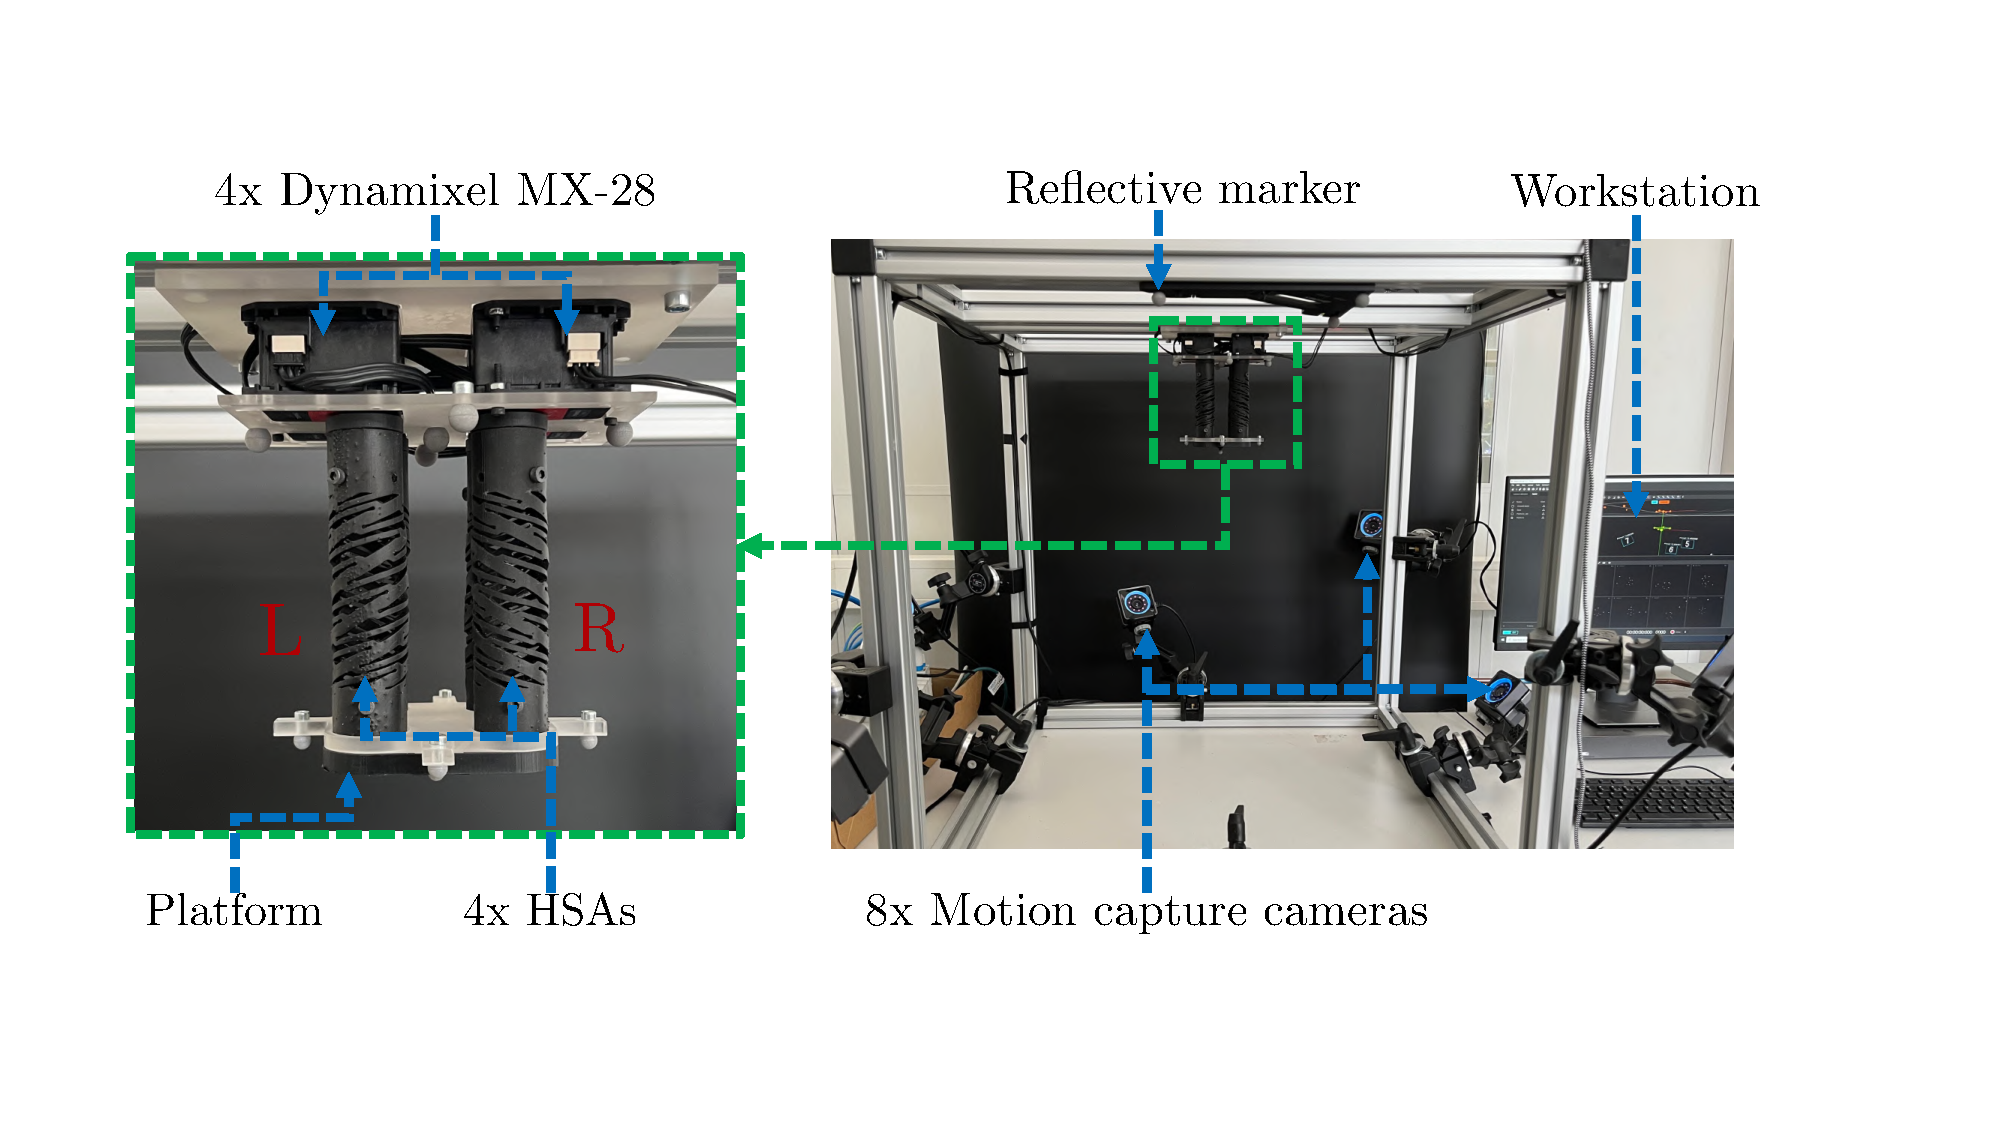
\includegraphics[width=0.85\textwidth]{hsacontrol/figures/experimental_setup_v2_cropped_compressed.pdf}
    \caption{Experimental setup: the parallel robot consists of four HSA rods connected by a platform at their distal end. Four servo motors actuate the HSAs. We track the pose of the end-effector with a motion capture system by attaching reflective markers to the platform.}
    \label{fig:hsacontrol:experimental_setup}
\end{figure}

\subsection{Experimental setup}\label{sub:hsacontrol:configuration_space_regulation:experimental_setup}
We evaluate the system model and our proposed control approach on a robot consisting of four HSA rods.
The material choice of the \gls{HSA} is crucial and has a significant influence on the resulting mechanical characteristics of the robot  (e.g., blocked force, holding torque, bending stiffness, etc.)~\cite{truby2021recipe}. Furthermore, specific material requirements are dictated by the nature of the design of the \gls{HSA} rod. The structure of the metamaterial is made of struts connected by living hinges. These living hinges must be thin, flexible, and accommodate high strains~\cite{truby2021recipe}.
Therefore, we decided to 3D-print the \glspl{HSA} via digital projection lithography either from the photopolymer resin Carbon FPU 50 (stiffer) or the elastomeric polyurethane EPU 40 resin (softer).
% citations for datasheets: ~\cite{carbon:fpu50} ~\cite{carbon:epu40}

Each \gls{HSA} rod is actuated by a Dynamixel MX-28 servo motor. The Dynamixel motors are set to use position control mode. % which runs a cascaded PID control loop on the motor current.
% The robot is mounted platform-down on a cage on which we have also attached eight Optitrack PrimeX 13 cameras. The motion capture system can track the SE(3) pose of both the base and the platform at a sampling rate of \SI{200}{Hz}. 
The robot is mounted platform-down on a cage with an Optitrack motion capture system, which measures the SE(3) pose of the platform at \SI{200}{Hz}.
Our algorithms run within a ROS2 framework\footnote{\url{https://github.com/tud-phi/ros2-hsa}}. % First, we project the pose measurements into the plane of actuation. Then, we evaluate the coordinate transformation between platform and base and run the closed-form inverse kinematics introduced in \eqref{eq:hsacontrol:kinematics}. We store in memory the last \textcolor{orange}{ten} configuration measurements, fit a cubic spline to each configuration variable using the \emph{Derivative} package~\cite{kaptanoglu2022pysindy}, and then differentiate the spline function to gather $\dot{q}(t)$.
% ~\footnote{\url{https://github.com/tud-phi/ros2-hsa}}
% ~\cite{kaptanoglu2022pysindy}
% Our algorithms run within a ROS2 framework. 
The pose measurements are first projected into the plane of actuation and serve as an input to the closed-form inverse kinematics introduced in \eqref{eq:hsamodel:planar_hsa_robot_model:kinematics}. 
We use a Savitzky-Golay filter with a window duration of $\SI{0.1}{s}$ to numerically differentiate $\chi_\mathrm{ee}(t)$, $q(t)$ and gather with that $\dot{\chi}_\mathrm{ee}(t)$ and $\dot{q}(t)$.
We fit a cubic spline to the last $16$ configuration measurements and differentiate~\cite{kaptanoglu2022pysindy} to gather $\dot{q}(t)$.


\subsection{System identification}
We follow the same system identification procedure as in Sec.~\ref{sub:hsamodel:planar_hsa_robot_model:model_verification}.
For the FPU-based robot, we identify $C_\varepsilon^\mathrm{FPU}=\SI{0.0079}{m \per rad}$, $S_\mathrm{be}^\mathrm{FPU} = -2.5 \cdot 10^{-5} + 3.9 \cdot 10^{-7} \, \frac{\phi_i^+}{l^0} \si{Nm^2}$, $S_\mathrm{sh}^\mathrm{FPU} = 0.043 + 0.0029 \, \frac{\phi_i^+}{l^0} \si{N}$, $S_\mathrm{ax}^\mathrm{FPU} = 0.74 + 0.0098 \, \frac{\phi_i^+}{l^0} \si{N}$, and $S_\mathrm{b,sh}^\mathrm{FPU} = -5.0 \cdot 10^{-4} \si{Nm \per rad}$ where $l^0 = \SI{0.059}{m}$. 
Furthermore, we regress $C_\varepsilon^\mathrm{EPU}=\SI{0.0098}{m \per rad}$, $S_\mathrm{be}^\mathrm{EPU} = 5.7 \cdot 10^{-4} -9.7 \cdot 10^{-6} \, \frac{\phi_i^+}{l^0} \si{Nm^2}$, $S_\mathrm{sh}^\mathrm{EPU} = 0.59 - 0.00047 \, \frac{\phi_i^+}{l^0} \si{N}$, $S_\mathrm{ax}^\mathrm{EPU} = 5.7 + 0.015 \, \frac{\phi_i^+}{l^0} \si{N}$, and $S_\mathrm{b,sh}^\mathrm{EPU} = -\SI{0.00048}{Nm \per rad}$ for the EPU \glspl{HSA} which have the same length as the FPU \glspl{HSA}.
Finally, we identify the axial rest strain $\sigma_\mathrm{ax}^0$ before the start of each experiment.

\begin{figure}[ht]
    \centering
    \subfigure[End-effector position]{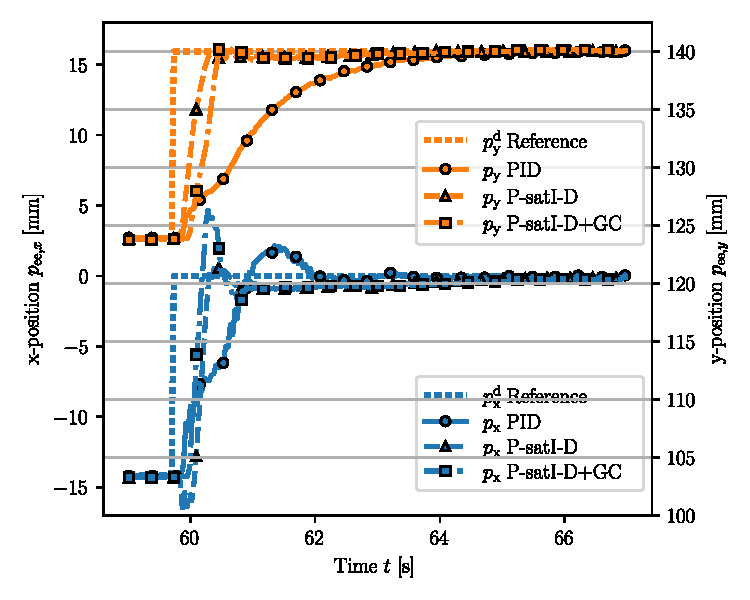
\includegraphics[width=0.49\columnwidth, trim={10, 10, 10, 10}]{hsacontrol/figures/experimental_results/configuration_space_regulation/fpu/fpu_step_response_chiee.pdf}\label{fig:hsacontrol:experimental_results:configuration_space_regulation:fpu:step_response:pee}}
    \subfigure[Configuration]{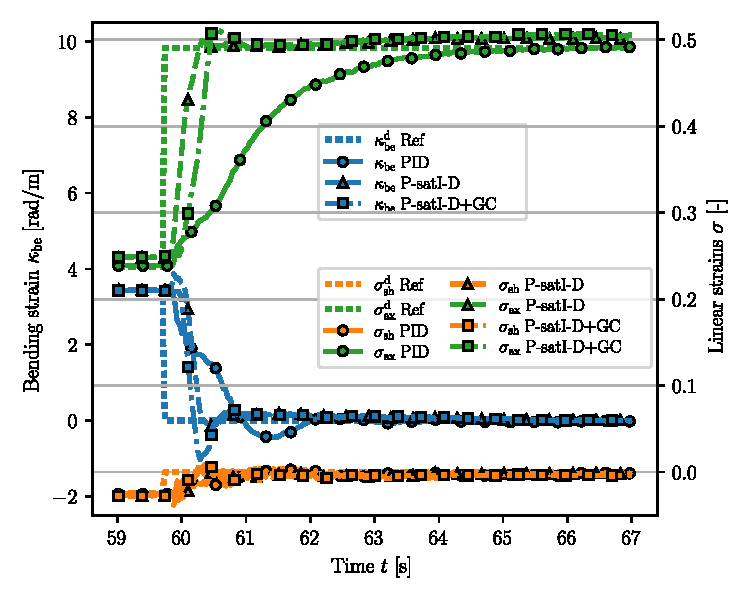
\includegraphics[width=0.49\columnwidth, trim={10, 10, 10, 10}]{hsacontrol/figures/experimental_results/configuration_space_regulation/fpu/fpu_step_response_q.pdf}\label{fig:hsacontrol:experimental_results:configuration_space_regulation:fpu:step_response:q}}
    \caption{Step response of the \emph{baseline PID}, \emph{P-satI-D} (with gravity compensation), and \emph{P-satI-D + GC} (with gravity cancellation) controllers on an FPU-based HSA robot.}\label{fig:hsacontrol:experimental_results:configuration_space_regulation:fpu:step_response}
\end{figure}

\begin{figure}[t]
    \centering
    \subfigure[End-effector position]{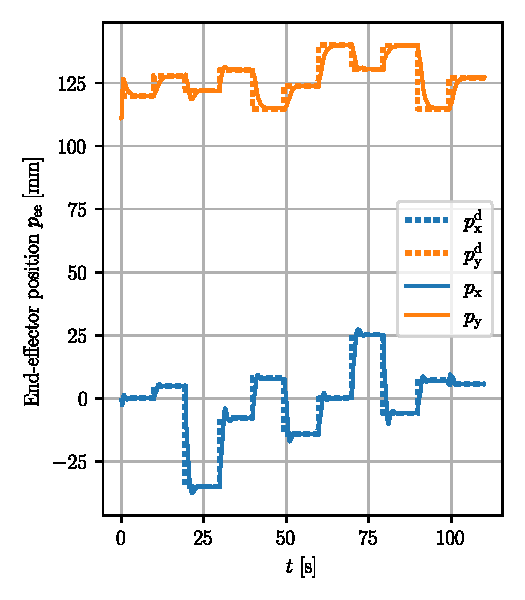
\includegraphics[width=0.32\columnwidth, trim={10, 10, 5, 10}]{hsacontrol/figures/experimental_results/configuration_space_regulation/fpu/20230925_092200_pee_three_panel_layout.pdf}\label{fig:hsacontrol:experimental_results:configuration_space_regulation:fpu:baseline_pid:pee}}
    \subfigure[Configuration]{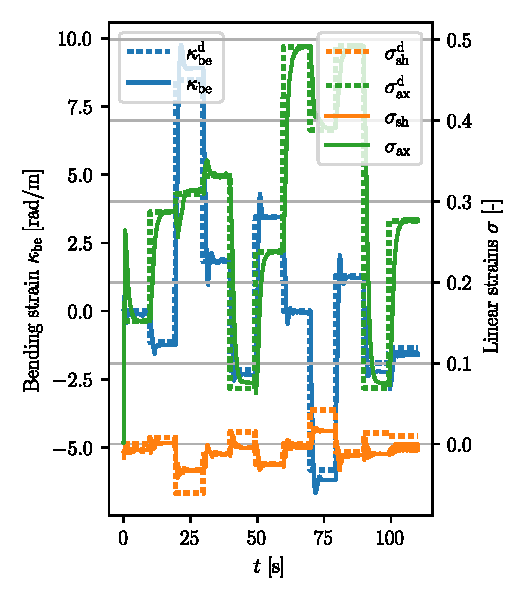
\includegraphics[width=0.32\columnwidth, trim={10, 10, 10, 10}]{hsacontrol/figures/experimental_results/configuration_space_regulation/fpu/20230925_092200_q_three_panel_layout.pdf}\label{fig:hsacontrol:experimental_results:configuration_space_regulation:fpu:baseline_pid:q}}
    \subfigure[Control input]{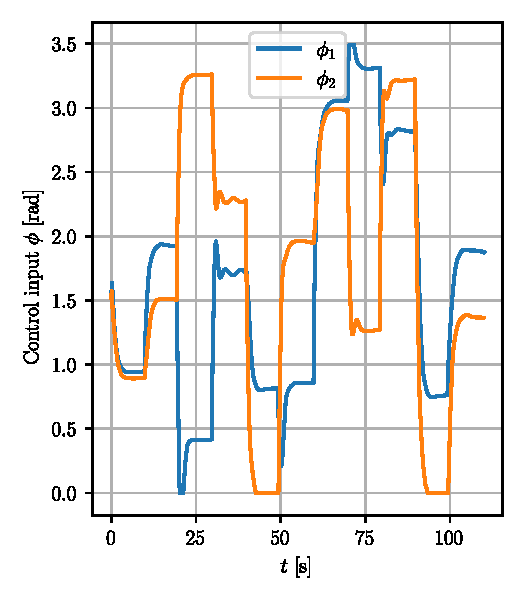
\includegraphics[width=0.32\columnwidth, trim={10, 10, 10, 10}]{hsacontrol/figures/experimental_results/configuration_space_regulation/fpu/20230925_092200_phi_three_panel_layout.pdf}\label{fig:hsacontrol:experimental_results:configuration_space_regulation:fpu:baseline_pid:phi}}
    \caption{Experimental results for tracking a reference trajectory of eleven step functions with the baseline PID controller on an FPU-based HSA robot. \textbf{Panel (a):} End-effector position with the dotted and solid lines denoting the task-space reference and actual position, respectively.
    \textbf{Panel (b):} The planned (dotted) and the actual (solid) configuration. 
    \textbf{Panel (c):} The planned (dotted) and the actual (solid) actuation coordinates of the collocated system. 
    \textbf{Panel(d):} The saturated planar control inputs are visualized with solid lines and the computed steady-state actuation with dotted lines.}\label{fig:hsacontrol:experimental_results:configuration_space_regulation:fpu:baseline_pid}
\end{figure}

\subsection{Implementation of closed-loop control}
Next, we implement the closed-loop control strategy laid out in Section~\ref{sub:hsacontrol:configuration_space_regulation:control_strategy}.
After evaluating the control law at a rate of \SI{40}{Hz} and saturating the control inputs to the ranges $[0, 3.40] \, \si{rad}$ for FPU and $[0, 4.71] \, \si{rad}$ for EPU, respectively, we map $\phi \in \mathbb{R}^2$ to desired positions of the four motors. For this, we consider the handedness of the \glspl{HSA} and apply the same actuation magnitude to both rods on the same side of the virtual backbone.
After tuning the gains for the feedback part of the model-based control laws in \eqref{eq:hsacontrol:gravity_compensation_controller} and \eqref{eq:hsacontrol:gravity_cancellation_controller}, we select $K_\mathrm{p} = \mathrm{diag}(0.3, 0.3)$, $K_\mathrm{i} = \mathrm{diag}(0.05, 0.05) \, \si{1 \per s}$, $K_\mathrm{d} = \mathrm{diag}(0.01, 0.01) \, \si{s}$, and $\gamma = \mathrm{diag}(100, 100)$. 
Furthermore, we report the performance of a model-free PID controller as a baseline. Here, the control input in task-space is given by $u_\mathrm{ts} = \begin{bmatrix}u_\mathrm{ts,x} & u_\mathrm{ts,y}\end{bmatrix}^\mathrm{T} = K_\mathrm{p}^\mathrm{PID} \, (p_\mathrm{ee}^\mathrm{d}-p_\mathrm{ee}) - K_\mathrm{d}^\mathrm{PID} \, \dot{p}_\mathrm{ee} + K_\mathrm{i}^\mathrm{PID} \int_0^t p_{\mathrm{ee},t'}^\mathrm{d} - p_{\mathrm{ee},t'} \: \mathrm{d}t'$, which is then mapped to the actuation via $\phi = \begin{bmatrix}
    u_\mathrm{ts,x}+u_\mathrm{ts,y}, & -u_\mathrm{ts,x}+u_\mathrm{ts,y}
\end{bmatrix}^\mathrm{T}$.
Here, we select $K_\mathrm{p}^\mathrm{PID} = \mathrm{diag}(10, 10) \, \si{rad \per m}$, $ K_\mathrm{i}^\mathrm{PID} = \mathrm{diag}(110, 110) \, \si{rad \per \meter \per \second}$, and $ K_\mathrm{d}^\mathrm{PID} = \mathrm{diag}(0.25, 0.25) \, \si{rad \, \second \per \meter}$.
\\

\begin{figure}[ht]
    \centering
    \subfigure[End-effector position]{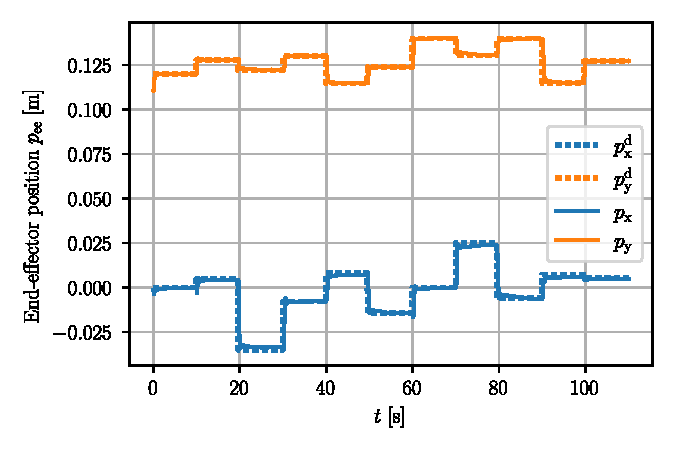
\includegraphics[width=0.49\columnwidth, trim={5, 10, 5, 5}]{hsacontrol/figures/experimental_results/configuration_space_regulation/fpu/20230925_093236_pee.pdf}\label{fig:hsacontrol:experimental_results:configuration_space_regulation:fpu:p_sati_d:pee}}
    \subfigure[Configuration]{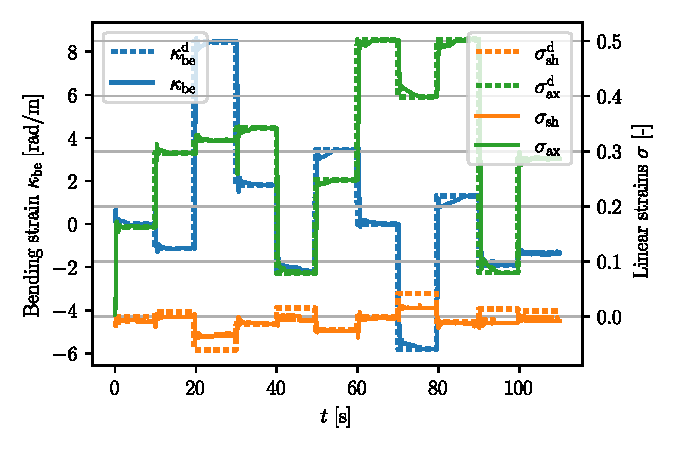
\includegraphics[width=0.49\columnwidth, trim={5, 10, 5, 5}]{hsacontrol/figures/experimental_results/configuration_space_regulation/fpu/20230925_093236_q.pdf}\label{fig:hsacontrol:experimental_results:configuration_space_regulation:fpu:p_sati_d:q}}\\
    \subfigure[Actuation coordinates]{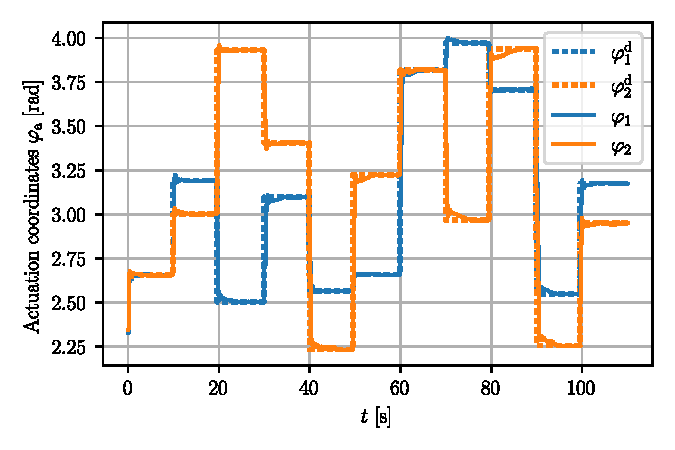
\includegraphics[width=0.49\columnwidth, trim={5, 10, 5, 5}]{hsacontrol/figures/experimental_results/configuration_space_regulation/fpu/20230925_093236_varphi.pdf}\label{fig:hsacontrol:experimental_results:configuration_space_regulation:fpu:p_sati_d:varphi}}
    \subfigure[Control input]{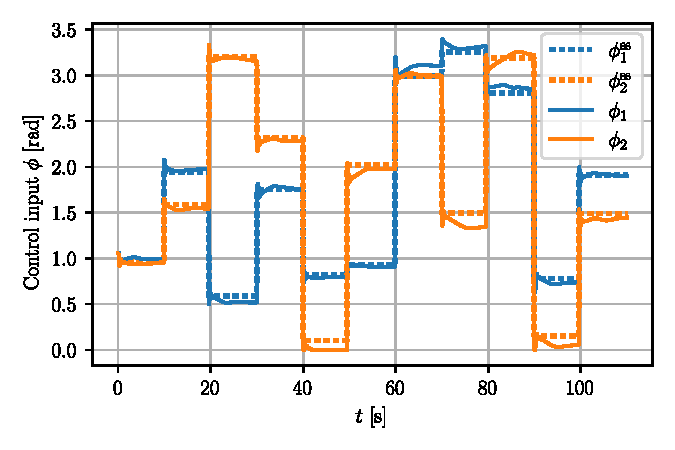
\includegraphics[width=0.49\columnwidth, trim={5, 10, 5, 5}]{hsacontrol/figures/experimental_results/configuration_space_regulation/fpu/20230925_093236_phi.pdf}\label{fig:hsacontrol:experimental_results:configuration_space_regulation:fpu:p_sati_d:phi}}\\
    \caption{Experimental results for tracking a reference trajectory of eleven step functions with the P-satI-D controller on an FPU-based HSA robot. \textbf{Panel (a):} End-effector position with the dotted and solid lines denoting the task-space reference and actual position, respectively.
    \textbf{Panel (b):} The planned (dotted) and the actual (solid) configuration. 
    \textbf{Panel (c):} The planned (dotted) and the actual (solid) actuation coordinates of the collocated system. 
    \textbf{Panel(d):} The saturated planar control inputs are visualized with solid lines and the computed steady-state actuation with dotted lines.}\label{fig:hsacontrol:experimental_results:configuration_space_regulation:fpu:p_sati_d}
\end{figure}

\begin{figure}[ht]
    \centering
    \subfigure[End-effector position]{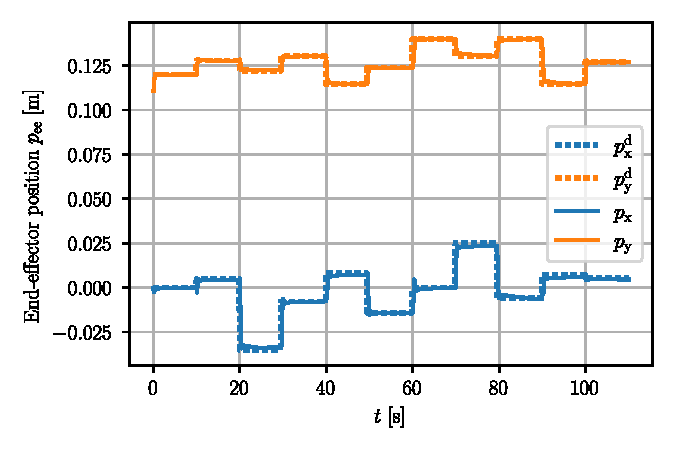
\includegraphics[width=0.49\columnwidth, trim={5, 5, 5, 5}]{hsacontrol/figures/experimental_results/configuration_space_regulation/fpu/20230925_094023_pee.pdf}\label{fig:hsacontrol:experimental_results:configuration_space_regulation:fpu:p_sati_d_plus_gc:pee}}
    \subfigure[Configuration]{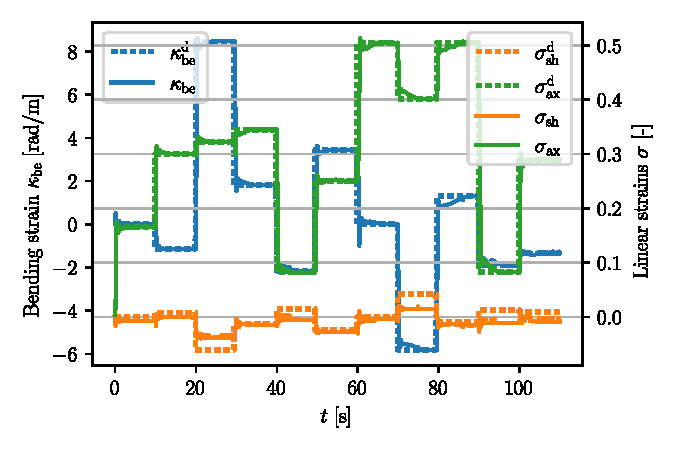
\includegraphics[width=0.49\columnwidth, trim={5, 5, 5, 5}]{hsacontrol/figures/experimental_results/configuration_space_regulation/fpu/20230925_094023_q.pdf}\label{fig:hsacontrol:experimental_results:configuration_space_regulation:fpu:p_sati_d_plus_gc:q}}\\
    \subfigure[Actuation coordinates]{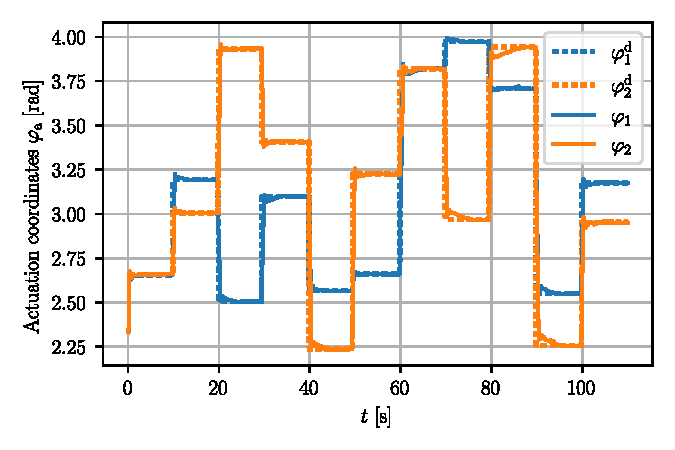
\includegraphics[width=0.49\columnwidth, trim={5, 5, 5, 5}]{hsacontrol/figures/experimental_results/configuration_space_regulation/fpu/20230925_094023_varphi.pdf}\label{fig:hsacontrol:experimental_results:configuration_space_regulation:fpu:p_sati_d_plus_gc:varphi}}
    \subfigure[Control input]{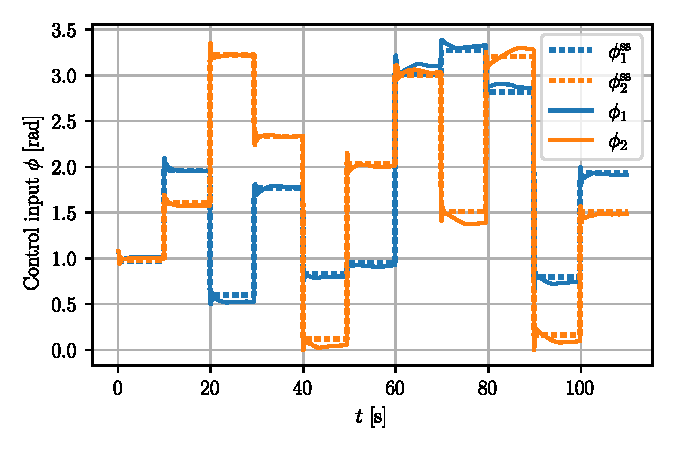
\includegraphics[width=0.49\columnwidth, trim={5, 5, 5, 5}]{hsacontrol/figures/experimental_results/configuration_space_regulation/fpu/20230925_094023_phi.pdf}\label{fig:hsacontrol:experimental_results:configuration_space_regulation:fpu:p_sati_d_plus_gc:phi}}\\
    \caption{Experimental results for tracking a reference trajectory of eleven step functions with the P-satI-D + gravity cancellation controller on an FPU-based HSA robot. \textbf{Panel (a):} End-effector position with the dotted and solid lines denoting the task-space reference and actual position, respectively.
    \textbf{Panel (b):} The planned (dotted) and the actual (solid) configuration. 
    \textbf{Panel (c):} The planned (dotted) and the actual (solid) actuation coordinates of the collocated system. 
    \textbf{Panel(d):} The saturated planar control inputs are visualized with solid lines and the computed steady-state actuation with dotted lines.}\label{fig:hsacontrol:experimental_results:configuration_space_regulation:fpu:p_sati_d_plus_gc}
\end{figure}

\subsection{Evaluation}
We define a reference trajectory $p_\mathrm{ee}^\mathrm{d}(k), k \in \{ 1, \dots, n_k \}$ with a duration of \SI{110}{s} and consisting of eleven step functions as the reference trajectory.
We report the \gls{RMSE} metric $\sqrt{\sum_{k=1}^{n_k} \frac{\lVert p_\mathrm{ee}^\mathrm{d}(k) - p_\mathrm{ee}(k) \rVert_2^2}{n_k}}$ for assessing the control performance, where $p_\mathrm{ee}(k)$ is the actual trajectory of the end-effector.\\

\subsection{Results for controlling an FPU-based HSA robot}
The \emph{baseline PID} achieves an \gls{RMSE} of \SI{5.86}{mm} with respect to the reference trajectory. The \emph{P-satI-D} based on \eqref{eq:hsacontrol:gravity_compensation_controller} (with gravity compensation) exhibits an RMSE of \SI{4.17}{mm}. Similarly, the \emph{P-satI-D + GC} based on \eqref{eq:hsacontrol:gravity_cancellation_controller} (with gravity cancellation) displays an RMSE of \SI{4.13}{mm}.
We present a comparison of the three different controllers for a step response in Fig.~\ref{fig:hsacontrol:experimental_results:configuration_space_regulation:fpu:step_response} and plot the entire trajectories of the \emph{baseline PID} and the \emph{P-satI-D} in Figures~\ref{fig:hsacontrol:experimental_results:configuration_space_regulation:fpu:baseline_pid} and \ref{fig:hsacontrol:experimental_results:configuration_space_regulation:fpu:p_sati_d}, respectively.
Additionally, we discretize various continuous reference trajectories into setpoints: 
star trajectory ($873$ setpoints and duration of \SI{109}{s}), the flame of the TU Delft logo ($680$ setpoints and duration of \SI{85}{s}), the contour of the MIT-CSAIL logo ($1046$ setpoints and duration of \SI{131}{s}), and the outline of a bat at three different sizes ($1510$ setpoints and \SI{189}{s} duration).
The resulting Cartesian evolutions of the \emph{P-satI-D} controller tracking these continuous references are displayed in Fig.~\ref{fig:hsacontrol:experimental_results:configuration_space_regulation:fpu:task_space_trajectories}.

\begin{figure}[ht]
    \centering
    \subfigure[Star]{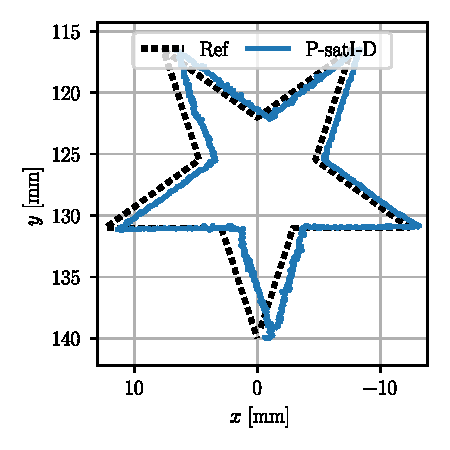
\includegraphics[width=0.32\columnwidth, trim={5, 5, 5, 5}]{hsacontrol/figures/experimental_results/configuration_space_regulation/fpu/20231019_072747_cartesian_evolution.pdf}\label{fig:hsacontrol:experimental_results:configuration_space_regulation:fpu:star}}
    \subfigure[TUD flame]{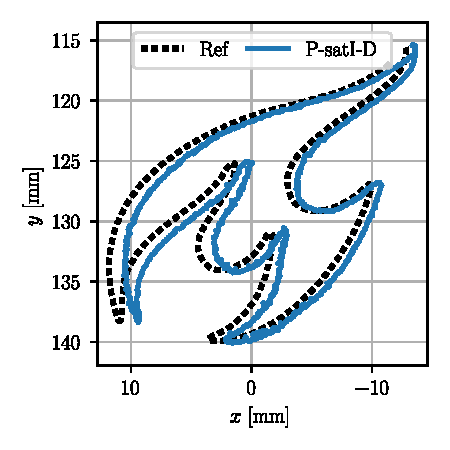
\includegraphics[width=0.32\columnwidth, trim={5, 5, 5, 5}]{hsacontrol/figures/experimental_results/configuration_space_regulation/fpu/20231019_081703_cartesian_evolution.pdf}\label{fig:hsacontrol:experimental_results:configuration_space_regulation:fpu:tud_flame}}
    \subfigure[MIT-CSAIL]{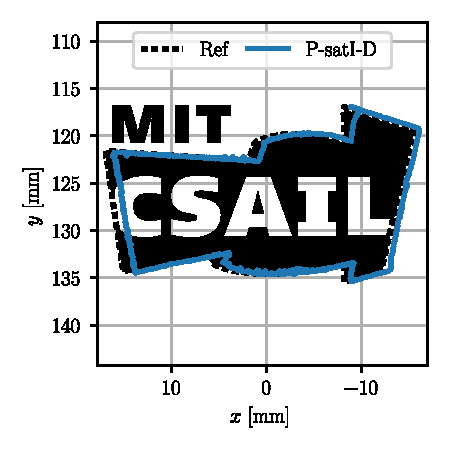
\includegraphics[width=0.32\columnwidth, trim={5, 5, 5, 5}]{hsacontrol/figures/experimental_results/configuration_space_regulation/fpu/20231019_082343_cartesian_evolution_with_logo.pdf}\label{fig:hsacontrol:experimental_results:configuration_space_regulation:fpu:mit_csail}}\\
    \subfigure[Bat trajectories]{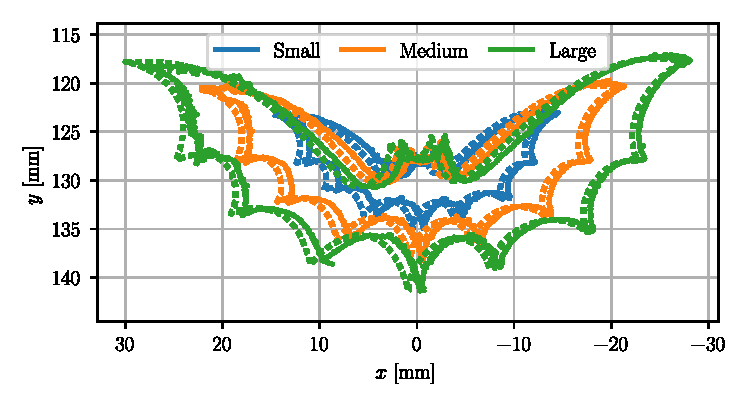
\includegraphics[width=0.7\columnwidth, trim={5, 5, 5, 5}]{hsacontrol/figures/experimental_results/configuration_space_regulation/fpu/fpu_bats.pdf}\label{fig:hsacontrol:experimental_results:configuration_space_regulation:fpu:bats}}
    \caption{Cartesian evolution of the proposed P-sat-D controller (solid lines) tracking various continuous reference trajectories (dotted lines) on the FPU robot.
    % we compare the performance of the baseline PID, the model-based P-satI-D controller (with gravity compensation), P-satI-D + GC which also includes terms to cancel the gravitational effects.
    }\label{fig:hsacontrol:experimental_results:configuration_space_regulation:fpu:task_space_trajectories}
\end{figure}

\begin{figure}[hb]
    \centering
    % each picture has a size 575x575px
    \subfigure[t=\SI{0}{s}]{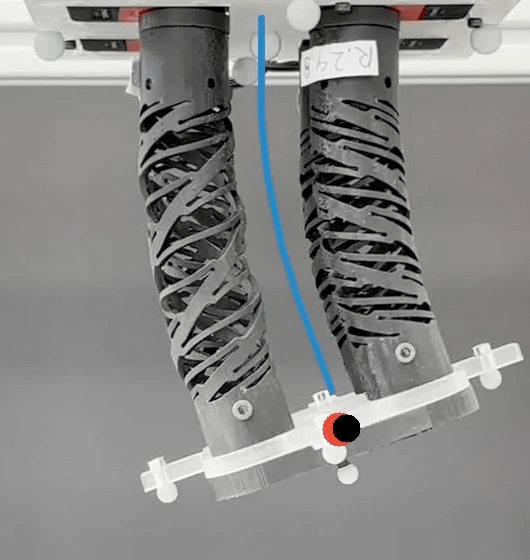
\includegraphics[width=0.192\columnwidth]{hsacontrol/figures/experimental_results/configuration_space_regulation/fpu/20231019_083240_overlayed_600x_cropped-0001-min.png}}
    \subfigure[t=\SI{47}{s}]{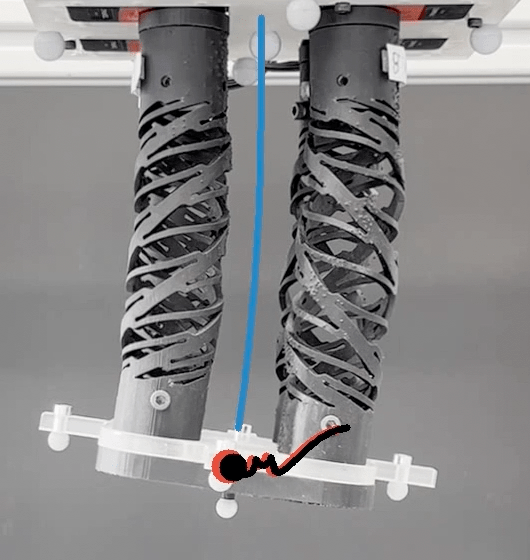
\includegraphics[width=0.192\columnwidth]{hsacontrol/figures/experimental_results/configuration_space_regulation/fpu/20231019_083240_overlayed_600x_cropped-0002-min.png}}
    \subfigure[t=\SI{94}{s}]{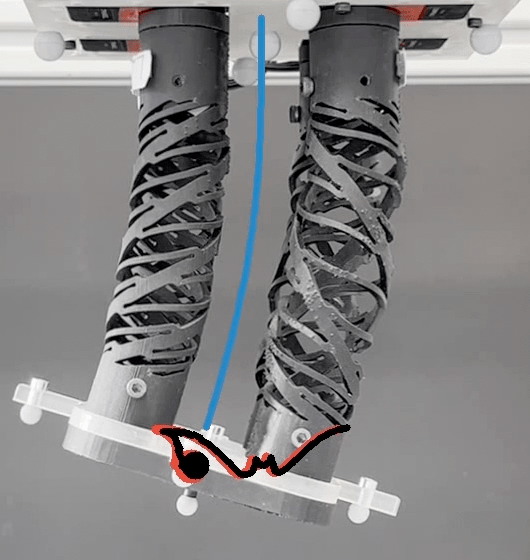
\includegraphics[width=0.192\columnwidth]{hsacontrol/figures/experimental_results/configuration_space_regulation/fpu/20231019_083240_overlayed_600x_cropped-0003-min.png}}
    \subfigure[t=\SI{141}{s}]{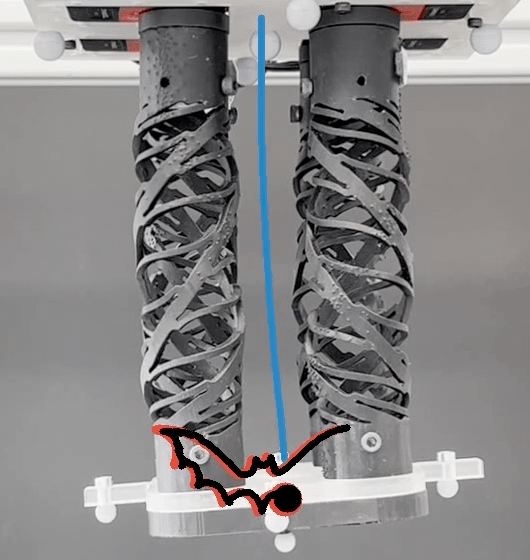
\includegraphics[width=0.192\columnwidth]{hsacontrol/figures/experimental_results/configuration_space_regulation/fpu/20231019_083240_overlayed_600x_cropped-0004-min.png}}
    \subfigure[t=\SI{188}{s}]{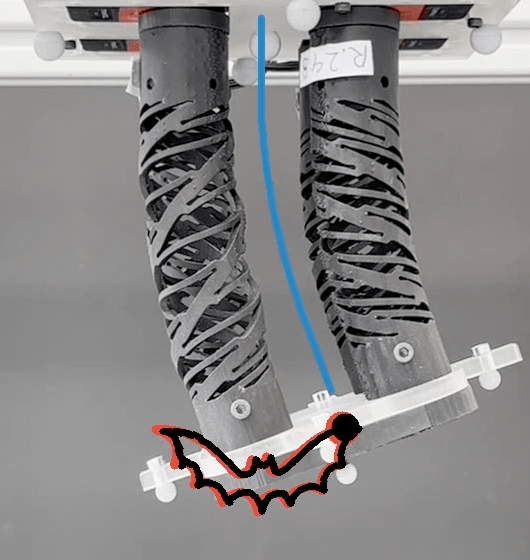
\includegraphics[width=0.192\columnwidth]{hsacontrol/figures/experimental_results/configuration_space_regulation/fpu/20231019_083240_overlayed_600x_cropped-0005-min.png}}
    \caption{Sequence of stills for the large bat trajectory performed with the P-satD controller on the FPU robot. The red and black dots visualize the desired and current end-effector positions, respectively. The past trajectory is plotted in red (reference) and black (actual). The blue line renders the shape of the virtual backbone.
    }\label{fig:hsacontrol:experimental_results:configuration_space_regulation:fpu:sequence_of_stills:bat}
\end{figure}

The step response in Fig.~\ref{fig:hsacontrol:experimental_results:configuration_space_regulation:fpu:step_response} shows how the two model-based controllers \emph{P-satI-D} and \emph{P-satI-D + GC} can leverage the planned $\phi^\mathrm{ss}$ and $q^\mathrm{d}$ to achieve a fast response time of roughly \SI{1.2}{s}. In contrast, the baseline PID needs to wait for the integral error to build up and thus has a much slower response time of approximately \SI{4.2}{s}. Furthermore, overshooting caused by the baseline PID is usually more extensive than that caused by the model-based controllers.
We conclude that \emph{P-satI-D} (gravity compensation) and \emph{P-satI-D + GC} (gravity cancellation) exhibit quite similar behavior. Sometimes, \emph{P-satI-D} exhibits undershooting at the beginning of the transient and \emph{P-satI-D + GC} overshooting towards the end of the transient (see Fig.~\ref{fig:hsacontrol:experimental_results:configuration_space_regulation:fpu:step_response:pee}).

\begin{figure}[ht]
    \centering
    \subfigure[End-effector position]{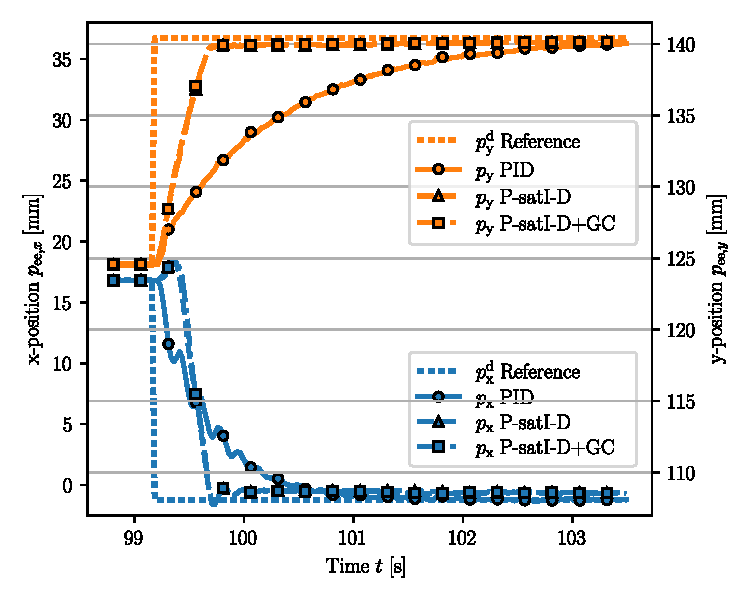
\includegraphics[width=0.47\columnwidth, trim={10, 10, 10, 10}]{hsacontrol/figures/experimental_results/configuration_space_regulation/epu/epu_step_response_chiee.pdf}\label{fig:hsacontrol:experimental_results:configuration_space_regulation:epu:step_response:pee}}
    \subfigure[Configuration]{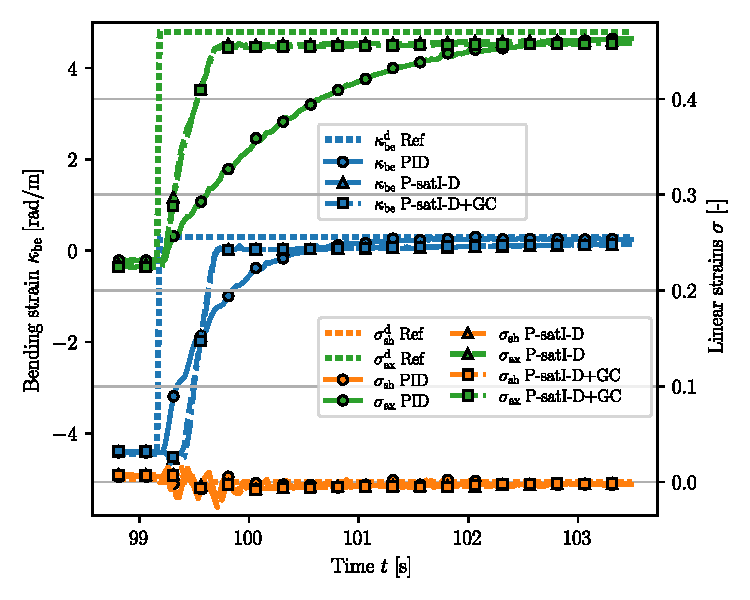
\includegraphics[width=0.47\columnwidth, trim={10, 10, 10, 10}]{hsacontrol/figures/experimental_results/configuration_space_regulation/epu/epu_step_response_q.pdf}\label{fig:hsacontrol:experimental_results:configuration_space_regulation:epu:step_response:q}}
    \caption{Step responses of the \emph{baseline PID}, \emph{P-satI-D} (with gravity compensation), and \emph{P-satI-D + GC} (with gravity cancellation) controllers on an EPU-based HSA robot.}\label{fig:hsacontrol:experimental_results:configuration_space_regulation:epu:step_response}
\end{figure}

\begin{figure}[ht]
    \centering
    \subfigure[End-effector position]{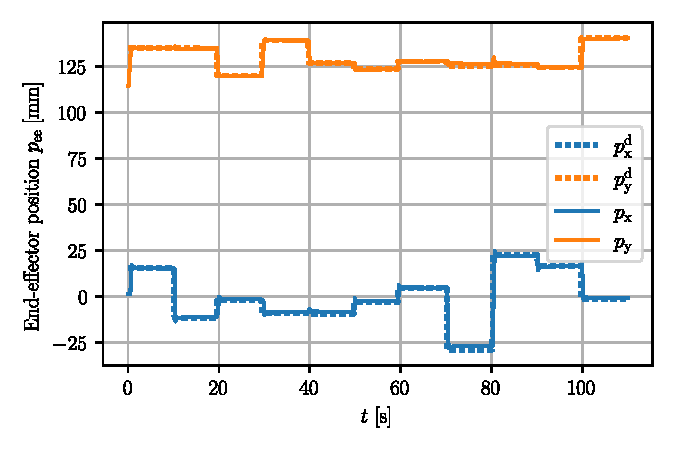
\includegraphics[width=0.49\columnwidth, trim={5, 10, 5, 5}]{hsacontrol/figures/experimental_results/configuration_space_regulation/epu/20231019_143126_pee.pdf}\label{fig:hsacontrol:experimental_results:configuration_space_regulation:epu:p_sati_d:pee}}
    \subfigure[Configuration]{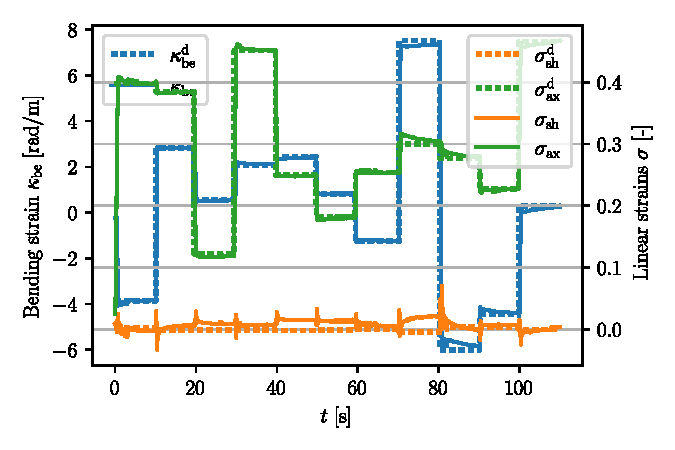
\includegraphics[width=0.49\columnwidth, trim={5, 10, 5, 5}]{hsacontrol/figures/experimental_results/configuration_space_regulation/epu/20231019_143126_q.pdf}\label{fig:hsacontrol:experimental_results:configuration_space_regulation:epu:p_sati_d:q}}\\
    \subfigure[Actuation coordinates]{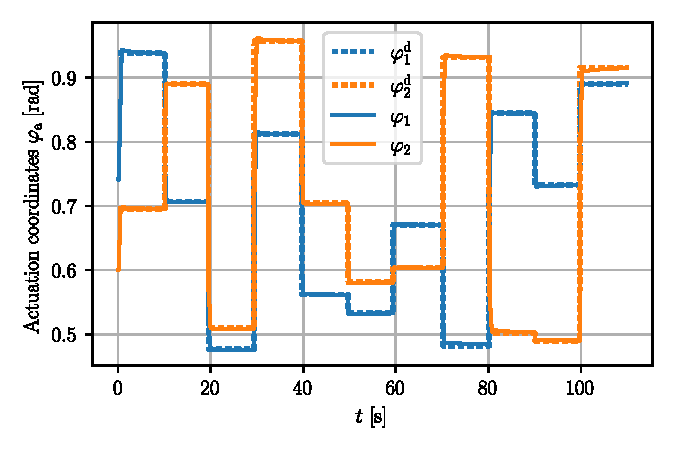
\includegraphics[width=0.49\columnwidth, trim={5, 10, 5, 5}]{hsacontrol/figures/experimental_results/configuration_space_regulation/epu/20231019_143126_varphi.pdf}\label{fig:hsacontrol:experimental_results:configuration_space_regulation:epu:p_sati_d:varphi}}
    \subfigure[Control input]{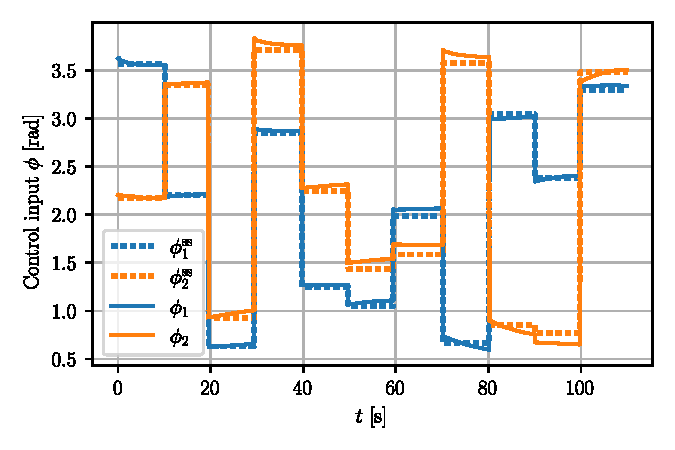
\includegraphics[width=0.49\columnwidth, trim={5, 10, 5, 5}]{hsacontrol/figures/experimental_results/configuration_space_regulation/epu/20231019_143126_phi.pdf}\label{fig:hsacontrol:experimental_results:configuration_space_regulation:epu:p_sati_d:phi}}
    \caption{Experimental results for tracking a reference trajectory of eleven step functions with the P-satI-D controller on an EPU-based HSA robot. \textbf{Panel (a):} End-effector position with the dotted and solid lines denoting the task-space reference and actual position, respectively.
    \textbf{Panel (b):} The planned (dotted) and the actual (solid) configuration. 
    \textbf{Panel (c):} The planned (dotted) and the actual (solid) actuation coordinates of the collocated system. 
    \textbf{Panel(d):} The saturated planar control inputs are visualized with solid lines and the computed steady-state actuation with dotted lines.}\label{fig:hsacontrol:experimental_results:configuration_space_regulation:epu:p_sati_d}
\end{figure}

\subsubsection{Results for controlling an EPU-based HSA robot}
Tracking the reference trajectory of eleven-step functions with an EPU-based robot, the \emph{baseline PID} controller has an \gls{RMSE} of \SI{4.40}{mm}. The \emph{P-satI-D} (with gravity compensation) can able to achieve an \gls{RMSE} of \SI{3.63}{mm}. The \emph{P-satI-D + GC} controller exhibits similar performance(\gls{RMSE} of \SI{3.71}{mm}).
We visualize the step response of all three controllers in Fig.~\ref{fig:hsacontrol:experimental_results:configuration_space_regulation:epu:step_response} and the entire trajectory of the \emph{P-satI-D} controller in Fig.~\ref{fig:hsacontrol:experimental_results:configuration_space_regulation:epu:p_sati_d}.

Again, we notice that the response time of the model-based controllers (\SI{0.54}{s}) is much shorter than the response time of the baseline PID (\SI{3.84}{s}). Furthermore, the importance of a model-based control law is motivated by the oscillations in the transient of the baseline PID (see x-coordinate in Fig.~\ref{fig:hsacontrol:experimental_results:configuration_space_regulation:epu:step_response:pee}).
The steady-state error for the model-based controllers on the EPU material is slightly higher compared to the FPU material, as seen in Figures \ref{fig:hsacontrol:experimental_results:configuration_space_regulation:epu:step_response:pee} \& \ref{fig:hsacontrol:experimental_results:configuration_space_regulation:epu:p_sati_d:pee}. In Section~\ref{sub:hsamodel:planar_hsa_robot_model:model_verification}, we noticed that the shear model doesn't fully capture the actual system behavior. This then results in an error in the planned desired configuration $q^\mathrm{d}$, which the controller is not able to resolve because of the underactuation of the robot (see Fig.~\ref{fig:hsacontrol:experimental_results:configuration_space_regulation:epu:p_sati_d:q}).
\section{Task-space impedance control}\label{sec:hsacontrol:task_space_impedance_control}
We introduce below a novel control strategy that addresses some limitations of the configuration-space regulation controller presented in Sec.~\ref{sub:hsacontrol:configuration_space_regulation:control_strategy} that are critically for achieving both structural and computational compliance. Namely, we (i) avoid computationally demanding planning procedures, (ii) remove integral terms that are unsafe for environment interaction, and (iii) enable impedance shaping in operational space. This Cartesian-space impedance controller is inspired by ~\cite{ott2008cartesian,della2020model}, but specifically designed for and tailored to \gls{HSA} robots. Crucially, we need to overcome the challenges of underactuation and the nonlinearity in the actuation - which were not present in that original work. %We, therefore, solve online a least-squares optimization problem, identifying the optimal actuation for generating the demanded task space forces.

\begin{figure}
    \centering
    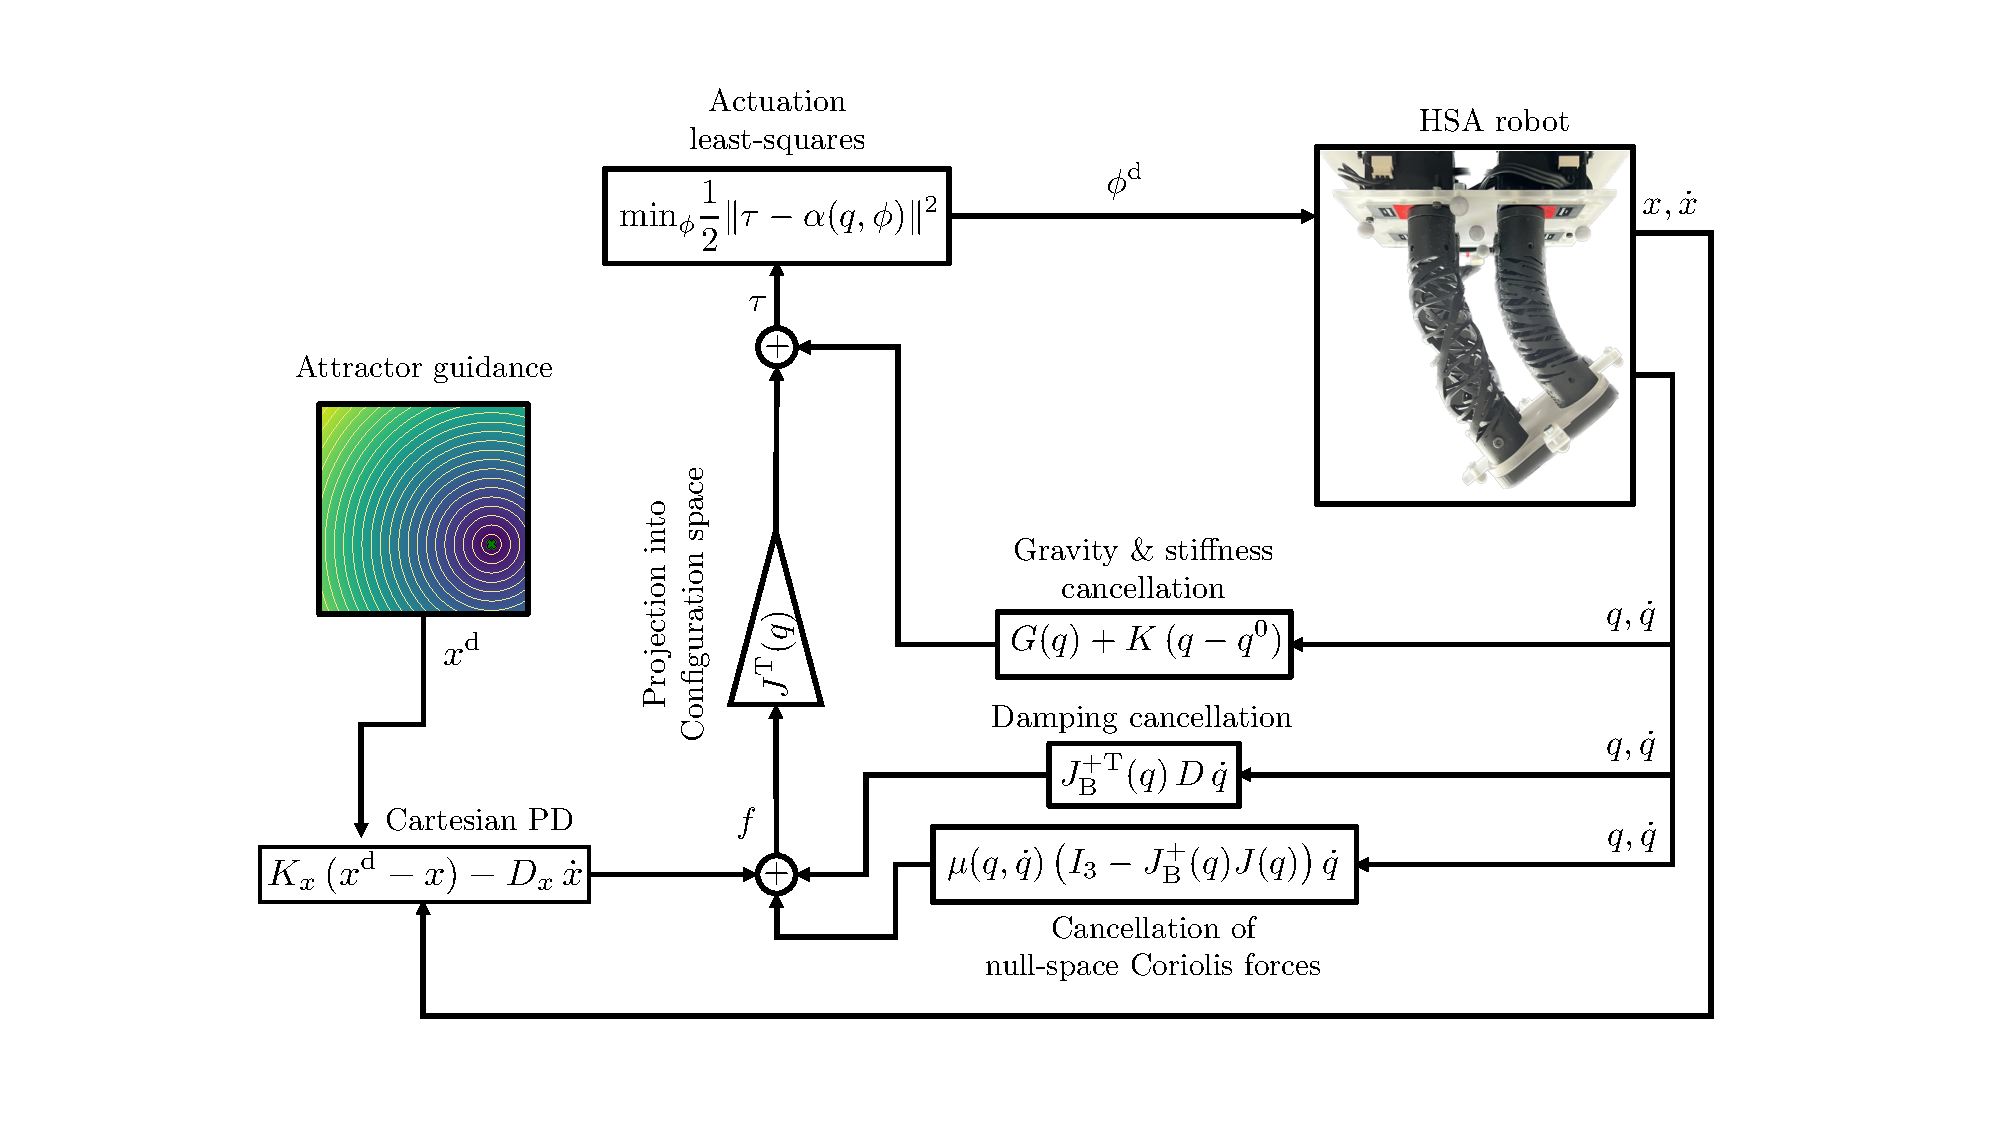
\includegraphics[width=0.9\textwidth]{hsacontrol/figures/control_schemes/cartesian_impedance_control/control_scheme_without_brain_control_cropped.pdf}
    \caption{Block scheme of the task-space impedance controller: after cancelling of the existing soft robot dynamics (e.g., null-space corioli forces, gravity, stiffness and damping), we reshape the potential field according to the desired Cartesian impedance $K_x, D_x$ with a globally asymptotically stable equilibrium at $x=x^\mathrm{d}$. Subsequently, we project the desired forcing $f$ from task-space to configuration-space. Finally, we solve a nonlinear least-squares optimization problem to match the desired configuration-space torques $\tau$ as closely as possible with the torques generated by the actuation $\phi^\mathrm{d}$.}
    \label{fig:hsacontrol:task_space_impedance_control:block_scheme_closed_loop_control}
\end{figure}

\subsection{Background: Task-space dynamics}\label{sub:hsacontrol:task_space_dynamics}
%
Although this has never been done in the context of HSA robots, it is immediate to see that their dynamics \eqref{eq:hsacontrol:dynamics} can be projected into operational space yielding the form~\cite{della2019exact, della2020model} % khatib1987unified
\begin{equation}\label{eq:hsacontrol:operational_space_dynamics}
    \Lambda(q) \, \Ddot{x} + \mu(q,\dot{q}) \dot{q} + J_\mathrm{B}^{+\mathrm{T}} ( G(q) + K (q-q^0) + D \, \dot{q} ) = J_\mathrm{B}^{+\mathrm{T}} \alpha(q,\phi),
\end{equation}
where $J_\mathrm{B}^+(q) = B^{-1}J^\mathrm{T}(J B^{-1} J^\mathrm{T})^{-1} \in \mathbb{R}^{3\times2}$ is the dynamically consistent pseudo-inverse, $\Lambda(q) = (J \, B^{-1} J^\mathrm{T})^{-1} \in \mathbb{R}^{2 \times 2}$ is the inertia matrix in task space, and $\mu(q, \dot{q}) = \Lambda(q) \, (J B^{-1} C - \dot{J}) \in \mathbb{R}^{2 \times 3}$ collects the Cartesian Coriolis and centrifugal terms. % ~\cite{khatib1987unified}

\subsection{Control strategy}\label{sub:hsacontrol:task_space_impedance_control:control_strategy}
% In previous work~\cite{stolzle2024experimental}, we have devised a model-based control strategy for regulating a planar \gls{HSA} robot towards a desired position in task space. %We propose here a new strategy that overcomes several limitations of that previous work which are critical for the application discussed in this chapter - namely: (i) it involves a complex and computationally demanding planning procedure for identifying a suitable setpoint in configuration space, (ii) our configuration-space controller contains integral terms, making it unsafe for environment interactions, and (iii) it is based on a compensation of static forces in configuration-space thus not allowing us to shape the impedance characteristics in operational space.
%
We will present the control strategy in two steps: first, we will introduce the control law and derive the associated desired configuration-space torques, and second, we will discuss how to map the control inputs to the actuation $\phi$.

\subsubsection{Proposed controller}
% We implement an operational space impedance action~\cite{ott2008cartesian, della2020model} that renders $x^\mathrm{d}$ an attractor of the closed-loop system.
We propose the following dynamic feedback law that renders $x^\mathrm{d}$ an attractor of the closed-loop system %~\cite{ott2008cartesian, della2020model} 
\begin{equation}\label{eq:hsacontrol:task_space_impedance_control:cartesian_impedance_controller}
\begin{split}
    \tau =& \: J^\mathrm{T}(q) \, \left (K_x \, (x^\mathrm{d} - x) - D_x \, \dot{x} \right ) + G(q) + K \, (q-q^0)\\
    & \: + J^\mathrm{T}(q) \, J_\mathrm{B}^{+\mathrm{T}}(q) \, D \, \dot{q} + J^\mathrm{T}(q) \, \mu(q,\dot{q}) \left ( I_3 - J_\mathrm{B}^+(q) J(q) \right )\dot{q}
\end{split}
\end{equation}
where $\tau \in \mathbb{R}^3$ is the desired torque in configuration space, $G(q) + K \, (q-q^0)$ cancels the acting gravitational and elastic forces, and $J^\mathrm{T} J_\mathrm{B}^{+\mathrm{T}} D \, \dot{q}$ removes the natural dissipation in operational space.
We emphasize that because the system is underactuated, we need to cancel the stiffness directly in the configuration instead of operational space as done in previous work~\cite{della2020model}.
We can shape our desired impedance characteristics in Cartesian space with the PD term $f_\mathrm{PD} = K_x \, (x^\mathrm{d} - x) - D_x \, \dot{x} $ which is then projected into configuration space by premultiplying with $J^\mathrm{T}(q)$.

The term $\mu(q,\dot{q}) \left ( I_3 - J_\mathrm{B}^+(q) J(q) \right )\dot{q}$ decouples the operational space dynamics from the residual of the null-space dynamics~\cite{della2020model}\cite[Ch. 4]{ott2008cartesian}.
The identity $\dot{q} = J_\mathrm{B}^+ \, \dot{x} + Z^\mathrm{T} \, \nu_\mathrm{N}$, where $Z^\mathrm{T} \in \mathbb{R}^{3 \times 1}$ is the dynamically-consistent pseudo-inverse of the null space, allows us to formulate $\dot{q}$ as a sum of the task-space velocity $\dot{x}$ and the null-space velocity $\nu_\mathrm{N}$. Leveraging this identity, the Coriolis and centrifugal matrix $\mu(q,\dot{q})$ can be split into a term $\mu_x(q,\dot{q}) = \mu \, J_\mathrm{B}^+ \in \mathbb{R}^{2 \times 2}$ excited by $x$ and the expression $\mu_\mathrm{N}(q,\dot{q}) = \mu \, Z^\mathrm{T} \in \mathbb{R}^{2 \times 1}$ that is excited by the null-space coordinates resulting in $\mu(q,\dot{q}) \, \dot{q} = \mu_x(q,\dot{q}) \, \dot{x} + \mu_\mathrm{N}(q,\dot{q}) \, \nu_\mathrm{N}$.
This allows us to cancel the term $\mu_\mathrm{N}(q,\dot{q}) \, \nu_\mathrm{N}$ through $\mu(q,\dot{q}) \left ( I_3 - J_\mathrm{B}^+(q) J(q) \right )\dot{q}$ without having to compute the null space explicitly.


% The first step consists of establishing a PD feedback in Cartesian space
% \begin{equation}
%     f =  K_x \, (x^\mathrm{d} - x) - D_x \, \dot{x} + J_\mathrm{B}^{+\mathrm{T}} \, D \, \dot{q}. % + \eta(q, \dot{q}) J_\mathrm{B}^+ \left (G(q) + K \, q \right ).
% \end{equation}
% where $K_x \in \mathbb{R}^{2\times2}$ is the designed task-space stiffness and $D_x % \in \mathbb{R}^{2\times2}$ adds dissipation.
% We make use of the kinematic Jacobian to project the designed task-space force into % configuration space and additionally establish cancellation of the gravitational and % elastic forces with
% \begin{equation}
%     \tau = \alpha(q,\phi) = J^\mathrm{T}(q) \, f + G(q) + K \, (q-q^0).
% \end{equation}

In summary, the closed-loop dynamics in operational space can be stated as
\begin{equation}\label{eq:hsacontrol:task_space_impedance_control:closed_loop_dynamics}
    \Lambda(q) \, \Ddot{x} + \mu(q,\dot{q}) \, J_\mathrm{B}^+ \, \dot{x} + K_x \, (x^\mathrm{d} - x) - D_x \, \dot{x} = 0,
\end{equation}
which results in $x^\mathrm{d}$ being the globally asymptotically stable equilibrium of the operational space dynamics.


\subsubsection{Mapping to actuation}
%
Now that we have formulated our control law $\tau$ in configuration space, we need to identify a strategy to specify the motor angles $\phi \in \mathbb{R}^2$ such that $\alpha(q,\phi) \approx \tau$. Note that, in contrast to other continuum soft robots studied in literature~\cite{della2023model}, the actuation term $\alpha(q,\phi)$ is not affine in control. %, but rather a nonlinear function with respect to the actuation coordinates $\phi$. 
%Therefore, mapping configuration-space torques to motor commands is not straightforward.
In previous work~\cite{stolzle2024experimental}, we side-stepped this challenge by linearizing with respect to the steady-state actuation $\phi^\mathrm{ss}$: $A(q) = \lVert \frac{\partial \alpha}{\partial \phi}\rVert_{\phi=\phi^\mathrm{ss}}$ therefore recovering the usual scenario of an affine actuation function. Unfortunately, this is not possible in the setting of this work as i) we do not have access to such $\phi^\mathrm{ss}$, and ii) linearizing around $\phi$ causes the closed-loop system to become unstable. We, therefore, propose to formulate instead a nonlinear least-squares problem $\phi^\mathrm{d} = \argmin_\phi \frac{1}{2} \lVert \tau - \alpha(q,\phi) \rVert^2$ and solve it in real-time with a Levenberg Marquardt solver implemented in JAX~\cite{jaxopt_implicit_diff}.

We note that this approach is not guaranteed to be valid for the general case of an underactuated soft robot but for this particular structure of $\alpha(q,\phi) \in \mathbb{R}^3$ with $\phi \in \mathbb{R}^2$ it is possible to identify solutions $\phi$ with the Euclidean norm of the residual being smaller than $0.001$.
The source code of the controller is available on GitHub\footnote{\url{https://github.com/tud-phi/hsa-planar-control}}.
% Next, the actuation vector is linearized with respect to the current twist angle $A_\phi(q) = \frac{\partial \alpha}{\partial \phi} \big|_{\phi} \in \mathbb{R}^{3 \times 2}$. With that, we now have
% \begin{equation}
%     J^\mathrm{T} f = \alpha(q,\phi) + A_\phi(q) \, u
% \end{equation}

\begin{figure}[t]
    \centering
    \subfigure[End-effector x-coordinate]{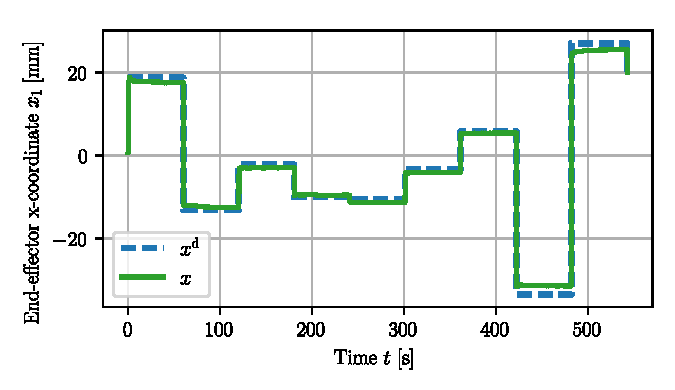
\includegraphics[width=0.47\textwidth, trim={5, 5, 5, 5}]{hsacontrol/figures/experimental_results/task_space_impedance_control/20231030_181558_pee_x.pdf}\label{fig:hsacontrol:experimental_results:task_space_impedance_control:pee_x}}
    \subfigure[End-effector y-coordinate]{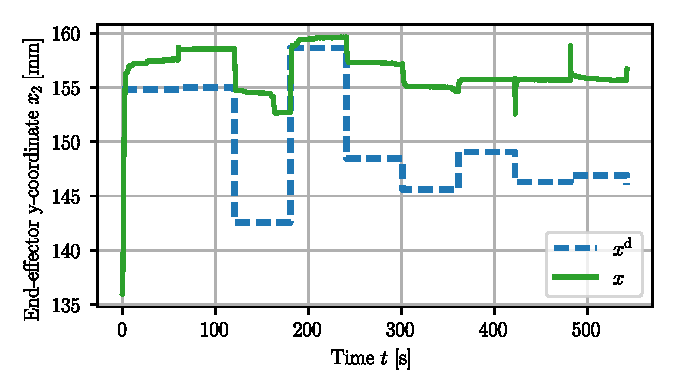
\includegraphics[width=0.47\textwidth, trim={5, 5, 5, 5}]{hsacontrol/figures/experimental_results/task_space_impedance_control/20231030_181558_pee_y.pdf}\label{fig:hsacontrol:experimental_results:task_space_impedance_control:pee_y}}\\
    \subfigure[Configuration $q$]{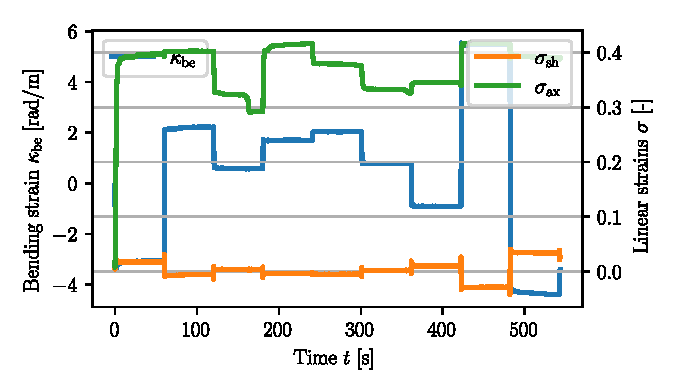
\includegraphics[width=0.47\textwidth, trim={5, 5, 5, 5}]{hsacontrol/figures/experimental_results/task_space_impedance_control/20231030_181558_q.pdf}\label{fig:hsacontrol:experimental_results:task_space_impedance_control:q}}
    \subfigure[Control input $\phi$]{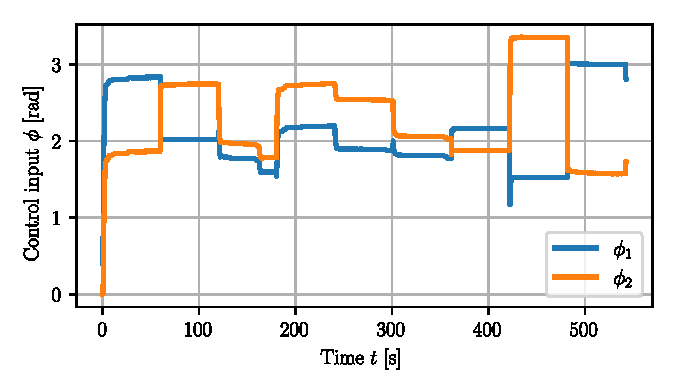
\includegraphics[width=0.47\textwidth, trim={5, 5, 5, 5}]{hsacontrol/figures/experimental_results/task_space_impedance_control/20231030_181558_phi.pdf}\label{fig:hsacontrol:experimental_results:task_space_impedance_control:phi}}
    \caption{Experimental results for tracking a reference trajectory of nine step functions with the Cartesian impedance controller. \textbf{Panel (a) \& (b):} The x/y-coordinate of the end-effector position with the solid line denoting the actual position, the dotted line the attractor position, and the dashed line the reference (i.e., the setpoint).
    \textbf{Panel (c):} The evolution of the configuration.
    \textbf{Panel(d):} The saturated planar control inputs. }\label{fig:hsacontrol:experimental_results:task_space_impedance_control}
\end{figure}

\subsection{Experimental setup}
We use the same experimental setup as introduced in Sec.~\ref{sub:hsacontrol:configuration_space_regulation:experimental_setup}.
Over a duration of \SI{540}{s}, we randomly generate nine setpoints $x^\mathrm{d}(t) \in \mathbb{R}^2$ within the operational workspace of the robot (see Fig.~\ref{fig:hsacontrol:kinematics:workspace}).
We evaluate the Cartesian impedance controller using the gains $K_\mathrm{p} = \SI{300}{N \per m}$, $K_\mathrm{d} = \SI{1.5}{N s \per \meter}$ at a frequency of \SI{50}{Hz} and finally send the desired motor positions to the servos.

% \subsection{Evaluation metrics}
% For evaluation purposes, we analyze the response time for reaching the proximity of the setpoint, which we define as $\lVert x^\mathrm{d} - x(t)\rVert_2 \leq \SI{2}{mm}$. Furthermore, we qualitatively assess the transient behavior of the system and the control input $\phi$.

\subsection{Results}
In Fig.~\ref{fig:hsacontrol:experimental_results:task_space_impedance_control}, we present the results of the experimental evaluation of the Cartesian impedance controller. 
The fast response time, a well-known characteristic of model-based control approaches, is evident. However, the errors in the model (for example, caused by hysteresis or unmodelled nonlinearities)~\cite{stolzle2024experimental}, together with the lack of integral action, lead to steady-state errors, whcih are especially pronounced for the y-coordinate.


\section{Experimental Insights}
This chapter presented two strategies for effective, model-based regulation of planar \gls{HSA} robots: the first proposes a configuration-space controller in conjunction with steady-state planning for mapping task-space setpoints to configuration-space setpoints, and the second introduces a task-space impedance controller.

\subsection{Configuration Space regulation}

First, we introduced a configuration-space controller that combines an integral-saturated PID controller with a potential-shaping feedforward term.
The excellent agreement of the model with the actual system behavior (as shown in Sec.~\ref{sec:hsamodel:planar_hsa_robot_model}) enables our model-based controllers to perform very well at the task of setpoint regulation.
For the model-based controllers, any mismatch between the dynamic model and the actual system (as analyzed in Section~\ref{sub:hsamodel:planar_hsa_robot_model:model_verification}) has two impacts: (i) the steady-state planning provides us with a desired configuration $q^\mathrm{d}$ which the underactuated robot cannot achieve. This then, in turn, causes a small steady-state error in the end-effector position as seen for the manual setpoints in Fig.~\ref{fig:hsacontrol:experimental_results:configuration_space_regulation:fpu:p_sati_d:pee} \& \ref{fig:hsacontrol:experimental_results:configuration_space_regulation:fpu:p_sati_d_plus_gc:pee} 
and for the continuous references in Fig.\ref{fig:hsacontrol:experimental_results:configuration_space_regulation:fpu:task_space_trajectories}. This steady-state error is absent in the baseline PID as its integral term acts directly in task space. We suggest that future work include an integral term directly on the end-effector position to remove the remaining steady-state error of the model-based controller. Secondly, as (ii), model errors will lead to an offset in the planned steady-state actuation $\phi^\mathrm{ss}$. Therefore, applying a constant $\phi^\mathrm{ss}$ will not move the robot exactly to $p_\mathrm{ee}^\mathrm{d}$. As shown in Fig.~\ref{fig:hsacontrol:experimental_results:configuration_space_regulation:fpu:p_sati_d:phi}, the P-satI-D feedback term can compensate for this effect through its proportional and integral terms applied in the collocated variables \& \ref{fig:hsacontrol:experimental_results:configuration_space_regulation:fpu:p_sati_d_plus_gc:phi} 
As clearly seen in Fig.~\ref{fig:hsacontrol:experimental_results:configuration_space_regulation:fpu:p_sati_d:phi}, the control input drifts away from the planned $\phi^\mathrm{ss}$ to counteract the modeling errors.
In particular, for small to medium bending and axial strains, we observe a very good agreement between the model and the actual system behavior and, therefore, excellent control performance. 
The story slightly changes for more significant bend and twist angles. While the system identification showed that the expressiveness of the model was sufficient, we saw significant errors in our feedforward terms in some of our control experiments, which needed to be compensated by the P-satI-D feedback controller. Precisely, Fig.~\ref{fig:hsacontrol:experimental_results:configuration_space_regulation:fpu:p_sati_d:q} displays errors in the planned shear strain, which subsequently also leads to minor steady-state deviations in the x-coordinate of the end-effector as it can be seen in Fig.~\ref{fig:hsacontrol:experimental_results:configuration_space_regulation:fpu:p_sati_d:pee}. We hypothesize that these errors are mainly caused by the hysteresis characteristics of the \glspl{HSA}~\citep{good2022expanding}. This hypothesis is corroborated by the fact that we had to re-calibrate the axial rest strain $\sigma_\mathrm{ax}^0$ before the start of each experiment.

\subsection{Task-space impedance control}
The Cartesian impedance controller, on the other hand, is designed to regulate the end-effector position directly and allows us to shape the impedance in task space and, with that, fully preserve the softness of the robot.
It is, therefore, particularly suitable for applications where the robot interacts with the environment. For example, we will in Chapter~\ref{chp:braincontrol} demonstrate how the impedance controller can be combined with motor-imagery brain signals to guide the robot towards a desired position and how the impedance controller guarantees safety even when the setpoints are wrongly planned.
This impedance needs to be traded off with steady-state errors. We observed that the impedance controller is particularly sensitive to the model errors, as it does not have an integral term to compensate for them.


\section*{Afterword}
This chapter presented the first control strategies in literature for \gls{HSA} robots and verified them experimentally on two \gls{HSA} robot prototypes in the planar case.
Each of the two presented controllers offers unique advantages:
On the one hand, the configuration-space P-satI-D + feedforward controller exhibits exceptional regulation accuracy, with minimal or no steady-state errors and exceptionally short response times.
On the other hand, the task-space impedance controller complements the passive compliance of the soft robot with active compliance in the control strategy. It accomplishes this by eliminating integral terms that could pose potential safety hazards. Additionally, it enables us to precisely shape the stiffness of the closed-loop system in Cartesian space.
% In this chapter, we programmatically specified the setpoints of the regulation controller. When working towards a future where soft robots assist, for example, elderly people with activities of daily living, we are lacking, however, an effective \gls{HRI} approach. A \gls{BMI} would arguably represent the most direct and barrier-free \gls{HRI} approach for assisting with activities of daily living. For that reason, we investigate in Chapter~\ref{chp:braincontrol} the guidance of the task-space impedance controller with \gls{EEG}-based motor imagery.
In envisioning a future where soft robots assist elderly individuals with activities of daily living, an effective \gls{HRI} is paramount. While this chapter has focused on programmatically specifying setpoints for regulation controllers, we recognize a gap in how humans can intuitively command these robots. A \gls{BMI} emerges as a compelling solution, offering a direct and barrier-free interaction method that could significantly enhance the usability of assistive robotics. Consequently, in Chapter~\ref{chp:braincontrol}, we explore the feasibility of guiding a task-space impedance controller via \gls{EEG}-based motor imagery, aiming to create a more natural and accessible means of control of soft, and specifically \gls{HSA}, robots.
Furthermore, we illustrate how the Cartesian-space stiffness enables us to apply force in the desired directions (in this case, releasing hairspray by pressing a button with the end-effector) while maintaining the compliance and, consequently, the embodied intelligence of the soft robot in all other directions.